\chapter{LITERATURE REVIEW}
\label{ch:litreview}

\section{Introduction}
This chapter will explore the current state of literature regarding the creation of Alunan, a mobile application designed to promote a vibrant online community among local musicians and enhance music exploration. This chapter provides a thorough analysis of the local music environment, focusing on notable trends, obstacles encountered by musicians, and successful music promotion tactics. This study examines the interactions within online communities, with a focus on content created by users and the integration of social media. Additionally, it investigates the process of discovering music, including the variety of genres and the influence of popular music streaming platforms. In addition, the chapter assesses different categories of mobile applications, emphasizing crucial characteristics and difficulties, thereby preparing for the eventual development of Alunan.

\section{Problem Domain}
The problem addressed in this literature review arises from apparent indicators within the local music scene. Local independent musicians encounter obstacles such as a divided web presence, insufficient representation, and a lack of suitable tools for exposure and marketing. These symptoms are worsened by the apparent issue of numerous separate websites and applications, a lack of features specifically designed for artists, and increased competition for attention in the digital domain. The absence of a specialized online community platform for local independent musicians poses a huge problem in this complex setting. There is currently a lack of a centralized platform for musicians to effectively connect, find opportunities, and get the necessary skills for navigating the music industry. \\

In the specific problem domain, previous studies provide additional understanding of the difficulties encountered by local independent musicians in the digital environment. \textcite{ong19} highlights the significance of social and cultural influences in the realm of musical expression, particularly the influence of alternative media, blogs, and websites on the formation of music communities. This highlights the significant impact of digital platforms in shaping the local music scene. \textcite{zanuar22} highlights the importance of social media platforms in marketing for independent artists, recognizing their effectiveness and the difficulties associated with operating within this realm. Gaining insight into how artists employ different social media platforms to interact with specific audience groups is essential for finding a solution to the problem area. Moreover, \textcite{edlom21} emphasizes the significance of fan communities in generating value for music companies, offering significant perspectives on the factors that drive fans to interact with musicians. Incorporating various viewpoints into the problem area improves the thorough comprehension necessary for the creation of Alunan, a specialized online community platform aimed at tackling the complex obstacles encountered by local independent musicians. \\

The proposed solution to this problem domain involves the creation of Alunan, a mobile application specifically tailored to tackle the observed symptoms and perceived concerns. Alunan seeks to enhance connections among local independent musicians by creating a dedicated internet platform, promoting increased visibility, and facilitating networking possibilities. The platform is designed to be an efficient platform that not only enables interaction but also supports the cultural and professional development of artists. Alunan aims to address the gaps in the problem domain by providing a comprehensive solution that caters to the specific requirements of local independent musicians in the constantly changing digital music industry.

\section{Local Musicians}
Local musicians are highly regarded in any community. These unsung music heroes perform in local hotels, tiny venues, and community events, sharing their love of music with their communities. These outstanding musicians lend a unique flavor to the local music industry by delivering a variety of styles and genres to suit their audience. Local musicians are storytellers who express their community's experiences, traditions, and emotions via their music. They become part of the local culture since their performances unite the audience. \\

According to \textcite{mohd21}, Local musicians in Malaysia play a crucial role in maintaining and promoting Malaysia's unique musical heritage. Malaysia's local singers serve as cultural ambassadors, representing the country's rich culture through the genres of Malay, Chinese, Indian, and indigenous music. They showcase the historical development of distinct Malaysian musical styles \parencite{mohd21}. By blending both traditional and modern sounds, they construct an evolving musical world that deeply connects with enthusiasts of music, establishing an inclusive identity where venues and events act as main places for gathering \parencite{ong19}. Malaysian musicians incorporate international musical trends while showcasing the nation's diverse heritage, encompassing traditional gamelan music to contemporary urban hip-hop. They perform at festivals, night markets, and cultural events, fostering solidarity among individuals from various origins through the unifying power of music in this global community.

\subsection{Types of Musicians}
\subsubsection{Independent Musicians}
According to \textcite{arditi21}, independent musicians represent an exclusive segment of the music business that does not receive backing from large record labels. These musicians are outstanding examples of self-sufficiency because they are in charge of independently overseeing all facets of their professions, from booking shows to handling finances. \textcite{martinez21} emphasizes, even more, how crucial social media is to independent bands' marketing campaigns. These musicians, who have total creative control over their songs and careers, use social media sites like Twitter and Instagram to promote themselves and interact with fans. These musicians' independence not only permits artistic freedom but also modifies the conventional dynamics of the music business by creating close relationships between performers and their audience.

\subsubsection{Hobbyist Musicians}
As stated by \textcite{arditi21}, hobbyist musicians represent a special category of the music industry. These people pursue music as a rewarding hobby rather than as their main source of income. The money they make from their musical endeavors is sometimes viewed as extra money, which sets them apart from professional musicians who rely only on their trade as a source of income. This distinction highlights the variety of reasons people listen to and participate in music; hobbyist musicians, for example, find joy and comfort in their work while continuing to pursue other primary sources of income or careers. This multimodal approach to music highlights its global appeal by allowing people to use it as an instrument for both personal expression and relaxation.

\subsubsection{Independent Label Musicians}
According to \textcite{arditi21} and \textcite{martinez21}, musicians who have ties with independent record labels are a unique group in the music business. These musicians enjoy a special set of benefits because they are signed to smaller labels that run independently from larger corporations. Independent labels give musicians more creative freedom over their music and career choices because they concentrate on more specialized genres or local specialties. This independence gives musicians the freedom to try out other genres and take unconventional approaches to production and marketing. In addition to enhancing artistic authenticity, the cooperative dynamic between musicians signed to independent labels and their smaller, more specialized associations adds to the energy and diversity of the music industry.

\subsubsection{Major Label Musicians}
As noted by \textcite{arditi21} and \textcite{martinez21}, musicians affiliated with large record labels play a crucial role in the music business. Major-label musicians have access to a wealth of marketing and promotional support because they are part of larger organizations with greater financial resources. This allows them to reach a worldwide audience. But working with big labels is not without its costs, as it frequently means giving up some creative freedom and control. Given that large labels place a premium on wider distribution and economic success, their influence over decisions about artistic direction and career choices is noteworthy. Major label musicians often gain public acclaim despite possible concessions, highlighting the delicate balance that these artists must strike in their careers between financial backing, artistic freedom, and industrial significance.

\subsubsection{Postlabel Musicians}
Post-label musicians represent an informed departure from the traditional form of recording contracts, in response to the issues highlighted by \textcite{arditi21}. These musicians have a more decentralized and independent approach, deliberately trying to avoid any exploitation by major labels. In the post-label era, musicians address the concerns that come with the possibility that signing a record label may result in a loss of artistic independence by placing a higher priority on retaining creative control and autonomy over their work. Post-label musicians move through the unstable music industry by utilizing independent distribution and digital platforms. They aim to establish a more fair and artist-focused model that confronts the possibility of exploitation that those who work in the conventional record label system may experience.

\subsection{Local Music Scene Trends}
\textcite{ong19} has observed that the local music scene in Malaysia has undergone substantial development in recent years, particularly in Kuala Lumpur, where a vibrant Indie Rock music community has emerged. This community prioritizes online connection and collaboration with the international and regional music scenes, promoting the development of independent labels that endorse regional Indie music. These labels offer a forum for musicians to produce music that departs from the worldwide popularised local rock and pop music genres. However, there are ongoing difficulties, mainly due to a lack of suitable locations for Indie Rock music performances. This issue has been further aggravated by the closing of major venues, resulting in a significant impact on the local Indie Rock music scene. Despite these obstacles, the community displays persistence by actively pursuing additional performing spaces and events that increase musical exposure and promote the development and endurance of local Indie Rock performers. \\

In addition, as emphasized by \textcite{mohd21}, the music industry in Malaysia has seen an engaging pattern of blending traditional Malaysian musical components with contemporary genres, resulting in a unique and varied musical environment. This fusion has not only gained popularity in Malaysia but has also attracted international acclaim, hence enhancing the global prominence of Malaysian music. Moreover, there is an emerging pattern of Malaysian artists engaging in partnerships with musicians from other countries, leading to the exchange of cultural elements and the integration of many musical influences into the domestic music landscape. This instance highlights the adaptability and creativity of Malaysian musicians in connecting different cultures through their music. \\

Furthermore, \textcite{silahudin19} has seen an increasing popularity of indie and alternative music genres in Malaysia, with local and worldwide acclaim being achieved by independent musicians and bands. This phenomenon has played a significant role in fostering a dynamic and varied music scene within the nation. In addition, Malaysian musicians have been engaging in the exploration of traditional sounds, combining them with modern elements to produce unique and different musical expressions. The expansion of digital platforms and social media has additionally furnished Malaysian musicians with fresh opportunities to exhibit their work, establish connections with listeners, and participate in partnerships with artists from various countries, leading to a more interconnected and globalized music scene in Malaysia. These trends collectively demonstrate the ever-changing and progressive nature of Malaysia's local music landscape. \pagebreak

\subsection{Local Music Scene Challenges}
The local music scene in Malaysia encounters substantial obstacles, mostly due to the lack of performance venues for Indie Rock music \parencite{ong19}. The closing of major venues has hurt the visibility of the local Indie Rock music scene, underscoring the urgent requirement for additional performance spaces and concerts that promote the development and longevity of local Indie Rock musicians. The limited number of available venues has presented challenges for musicians and organizers, limiting the growth and visibility of Indie Rock music in the local music scene. \\

In addition, as highlighted by \textcite{mohd21}, the music industry in Malaysia has numerous challenges. A notable obstacle comes in the attempt of local artists to acquire exposure and recognition in the highly competitive industry. The lack of resources and opportunities for independent musicians, coupled with the growing popularity of mainstream commercial music, present significant challenges to the development of the local music scene. Moreover, the problems associated with music piracy and copyright infringement have significantly affected the financial well-being of musicians and the long-term survival of the music industry in Malaysia. These challenges emphasize the necessity for increased assistance for the development and promotion of talents within the local music scene. \\

Furthermore, the music industry in Malaysia encounters specific challenges. An important obstacle is the insufficient assistance and promotion available to native musicians, particularly those who produce music in native languages or dialects \parencite{silahudin19}. This presents an obstacle to the preservation and development of Malaysia's diverse musical legacy. Moreover, the growing popularity of popular commercial music and global music trends could surpass the importance of local talents, posing a challenge for up-and-coming Malaysian artists to establish themselves in the industry. Moreover, the pressing concerns of copyright protection, fair compensation, and sustainable income for artists in the digital age emphasize the necessity for improved support structures to guarantee the livelihood of traditional music artists in Malaysia.

\subsection{Electronic Press Kit}
\begin{figure}[h]
  \centering
  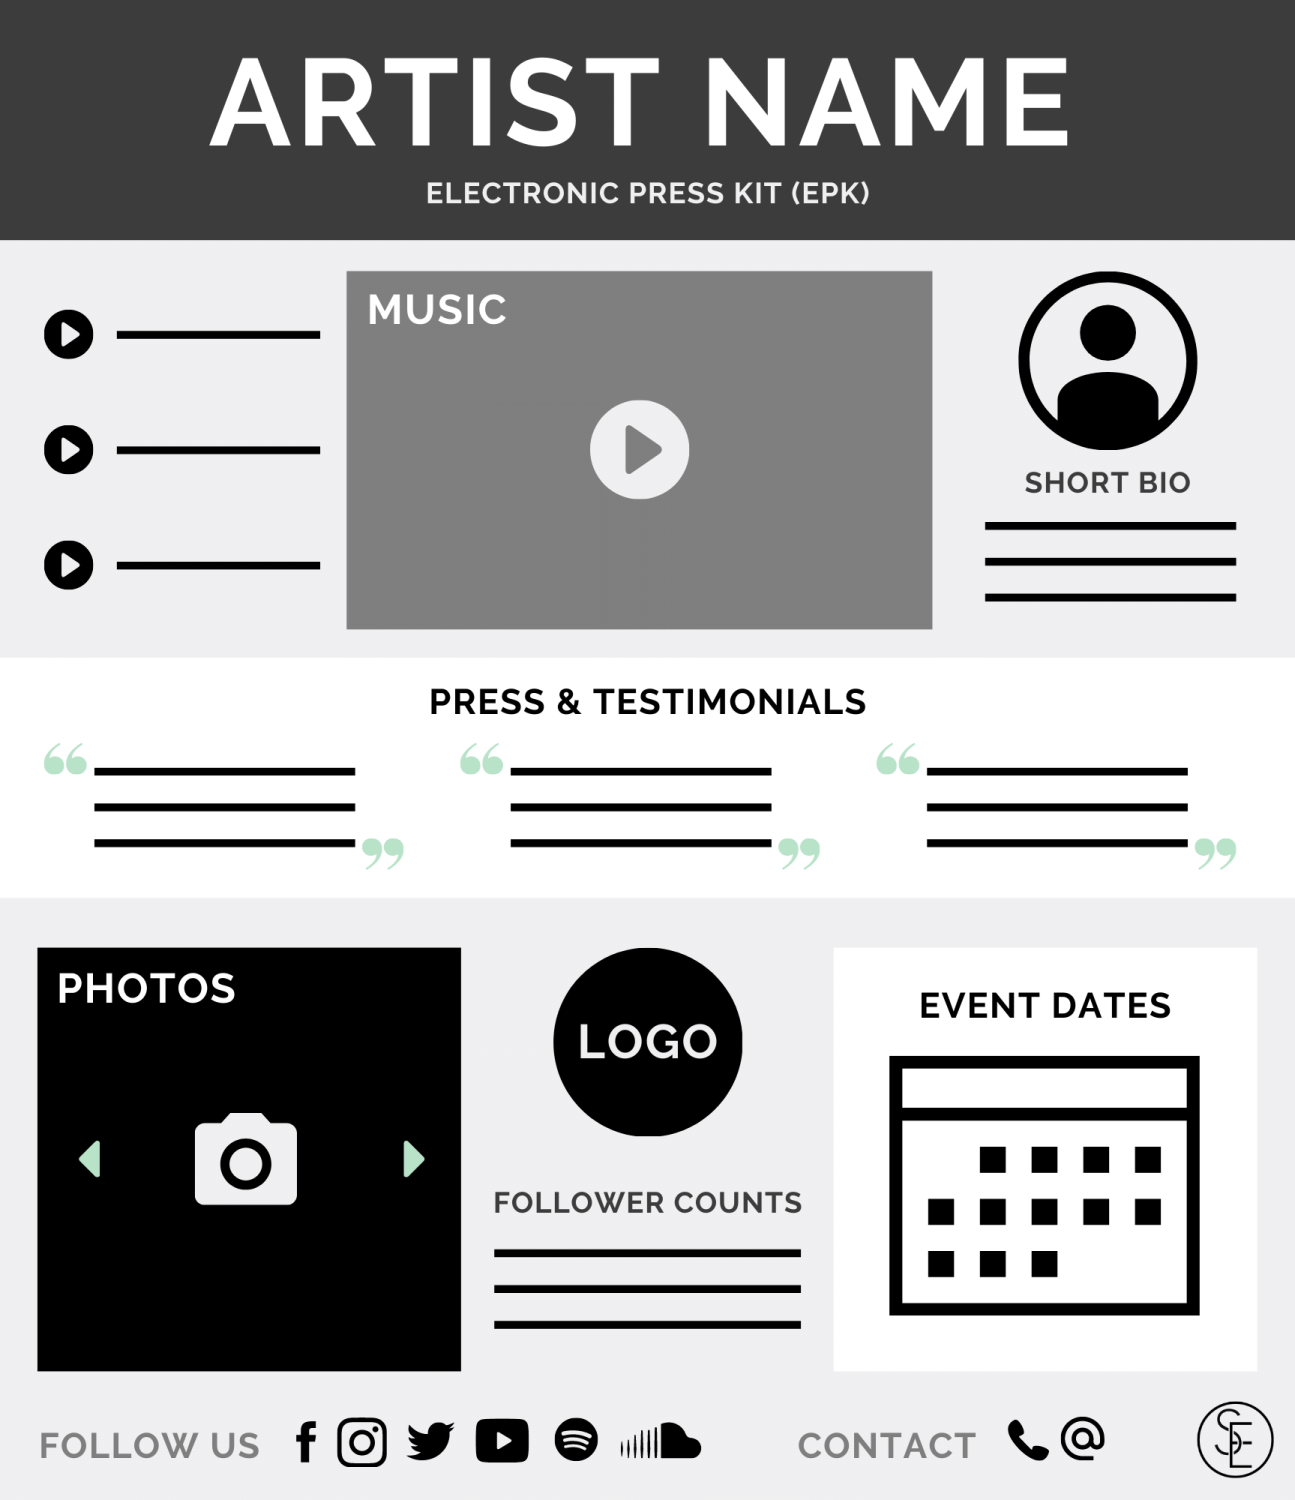
\includegraphics[width=0.45\linewidth]{mainmatter/images/epk.png}
  \caption{Template of Electronic Press Kit}
  \caption*{\textit{Electronic Press Kit 101: Why an EPK is Vital for Every Artist (2020, August 3)}}
  \caption*{https://www.linkedin.com/pulse/electronic-press-kit-101-why-epk-vital-every-artist-tyler-schurb/}
  \label{fig:myfig29}
\end{figure}
An electronic press kit (EPK) is a crucial promotional tool for musicians aiming to showcase their skills and capture the interest of industry experts, media platforms, and prospective supporters. An EPK, or electronic press kit, is a digital compilation of essential information about an artist presented in a user-friendly and easily accessible way, as opposed to traditional physical press kits. EPKs, as emphasized by \textcite{wilson20}, serve as a customized tool for artists and bands to tell their stories to booking agents, tour managers, record labels, and radio stations. The objective is to obtain opportunities such as performances, interviews, and contracts. The EPK, similar to a concise downloadable publication, contains essential details about the artist, with a particular emphasis on visually appealing aspects such as high-quality images. These photographs should not only prioritize resolution but also emphasize captivating composition. \pagebreak

An EPK often consists of a well-constructed biography that showcases the musician's background, influences, and notable achievements. Additionally, it showcases top-notch promotional photographs, guaranteeing a visually captivating portrayal of the artist. The EPK should exhibit the artist's musical expertise through audio and visual materials, such as sample tracks, music videos, or live performance footage. By employing an interactive method, industry specialists can promptly evaluate the artist's artistic style and prospects. In addition, the EPK includes essential social media links, emphasizing the crucial importance of having an online presence in the modern era. Moreover, the inclusion of direct hyperlinks to the artist's music, highlights the significance of making the music easily available to listeners, regardless of its quality, as a crucial factor for achieving success \parencite{wilson20}. In general, an electronic press kit functions as a thorough and adaptable tool, enabling musicians to create a memorable impact in the highly saturated music market.

\section{Online Community}
An online community is described as a digital space where individuals who have similar interests, objectives, or affiliations gather to communicate, share information, and participate in discussions or activities. Communities may exist in diverse formats, including forums, social media groups, or specialized platforms, offering members a virtual space to communicate, cooperate, and develop connections without being constrained by geographical limitations. Online community platforms such as Facebook Groups, Reddit, LinkedIn Groups, Discord servers, and niche-specific forums like Stack Overflow for programming enthusiasts or GitHub for software developers serve as examples. These platforms enable the establishment of communities centered around diverse subjects, spanning from personal interests and professional connections to mutual aid organizations and enthusiast associations. \pagebreak

\subsection{User-Generated Content}
According to \textcite{v22}, User-Generated Content (UGC) in online communities offers a diverse range of values, including functional, emotional, and social components. Functionally, user-generated content (UGC) frequently functions as a valuable source of information, guidance, and resolutions for members of a community. Emotionally, it cultivates a feeling of inclusion and mutual experiences, fostering emotional bonds among users. From a social perspective, user-generated content (UGC) plays a significant role in encouraging the development of a unified community, where individuals join based on common interests or objectives. This multidimensional value enhances participation and connection among community members. \\

The trust-building influence of user-generated content (UGC) in digital media, which is favored above traditional advertising \parencite{v22}. UGC is characterized by its authenticity, making it widely regarded as more genuine and reliable compared to content produced by professionals. Online communities place high importance on the thoughts and experiences given by their members, acknowledging them as genuine and trustworthy sources. The confidence and authority that is built through User-Generated Content (UGC) significantly impact the dynamics of a community and the level of influence its members have. \\

The quality of user-generated content (UGC) in online communities is impacted by multiple factors, as outlined by \textcite{luca21}. These elements include promotional content, peer effects, biases, and self-selection. UGC of superior quality frequently arises when individuals are driven by non-monetary incentives, such as badges or social standing, to provide excellent content to the community. These incentives can guide user contributions in a good manner, promoting the development of significant and influential content \parencite{luca21}. Hence, the interaction between the standard of content and the motivating factors has an important effect on the structure of user-generated content inside digital media platforms.\pagebreak

\begin{figure}[h]
    \centering
    
\includegraphics[width=0.9\linewidth]{mainmatter/images/ugc1.png}
    \caption{User-Generated Content (UGC) in TikTok}
    \caption*{\textit{TikTok post by @josephro53 (2021, June 22) [ByteDance, 2023]}}
    \label{fig:myfig3}
\end{figure}
Within the realm of user-generated material in online communities, it is useful to analyze two illustrative examples that demonstrate its influence and variety. The first figure involves a TikTok video review conducted by user @josephro53, which explores the realm of those who hold a deep passion and knowledge about sneakers. This user-generated material has a reviewer who offers a perceptive and subjective evaluation of the Makerz Rentaka sneakers. This content provides analytic value to viewers seeking product knowledge and a sense of connection with fellow sneaker enthusiasts who share a passion for the topic. \pagebreak

\begin{figure}[h]
    \centering
    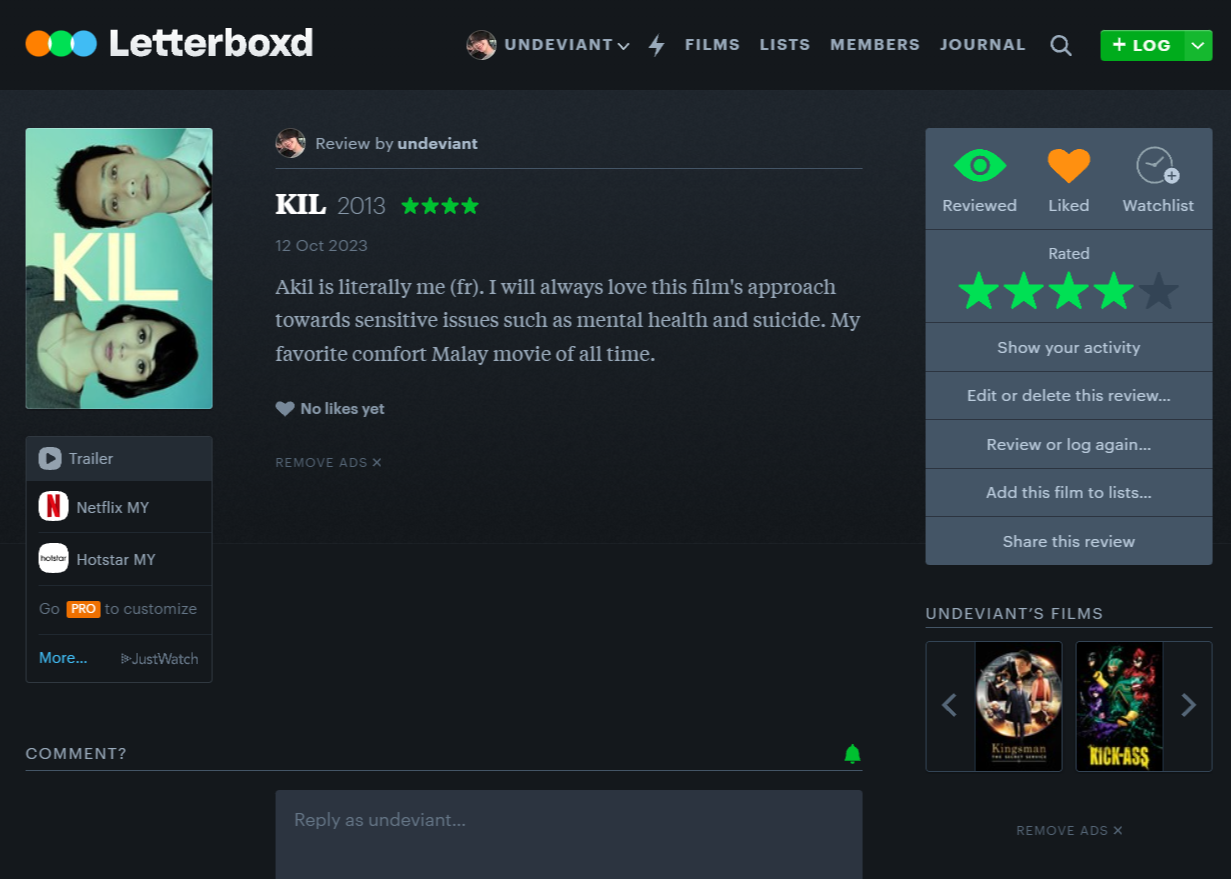
\includegraphics[width=0.8\linewidth]{mainmatter/images/ugc2.png}
    \caption{User-Generated Content (UGC) in Letterboxd}
    \caption*{\textit{Letterboxd post by @undeviant (2023, October 12) [Letterboxd, 2023]}}
    \label{fig:myfig4}
\end{figure}
The second figure, a movie review of "KIL (2013)" by user @undeviant on Letterboxd, illustrates the significance of user-generated content (UGC) in the area of cinema critique and admiration. In this review contributed by @undeviant, a perceptive evaluation of the Malaysian movie is presented, presenting an original viewpoint that enhances the discussion about the film. This material represents the trust and authority that users give to other community members when they are looking for recommendations or insights in their areas of interest.

\subsection{Social Media Integration}
The integration of social media into online communities has become an essential feature of modern digital interactions. This integration utilizes the capabilities of platforms such as Facebook, Twitter, and Instagram to improve the overall community experience. Online communities promote enhanced user involvement and exposure by enabling the seamless linking of social media profiles and content sharing. Integrating social media not only expands the audience for community content, but also promotes immediate conversations, exchange of valuable knowledge, and fast distribution of information \parencite{zanuar22}. This technology bridges the boundaries between virtual communities and the wider online social environment, allowing members to easily interact, cooperate, and contribute across several platforms, hence enhancing the overall community experience.

\subsection{Types of Interaction}
Interactions in online communities are complex and diverse, with different forms that each have their importance. Primarily, likes and reactions provide members with a convenient and efficient means to show their approval or appreciation for a post or comment. These confirming actions aim to inspire content authors and communicate that their efforts are highly esteemed in the community. Moreover, comments serve as the vital essence of discussions, offering a platform for individuals to express their opinions, pose inquiries, and participate in important conversations. Comment threads frequently develop into rich sources of knowledge, deep opinions, and varied points of view, promoting a feeling of community unity. \\

Sharing content is a crucial method for interaction within internet communities. When a member shares a post or discussion topic, it expands the visibility of that information to a wider audience, potentially recruiting new members and improving the overall reach of the community. Upvotes and downvotes, frequently observed on sites such as Reddit, allow users to indicate their approval or disapproval of particular posts or comments. This voting method helps the curation of content, guaranteeing that the most relevant and significant contributions rise to popularity, while irrelevant or improper content is dismissed. Furthermore, ratings and reviews have a crucial significance, particularly among communities that prioritize items, services, or information. Users can allocate ratings and submit comprehensive reviews, providing essential input and impacting the decisions of others. These assessments enhance knowledge and assist members in selecting the best services. \\

In addition to these interactions, mentions and tags play a crucial role in engaging particular community members in discussions and recognizing their expertise. Direct messaging enables confidential individual conversation, but polls and surveys provide a systematic approach to collecting community comments, opinions, or preferences. Emojis and reaction buttons serve to enhance the expression of emotions and sentiments towards content, providing additional depth and subtlety. These various types of interaction collectively enhance the overall experience of online communities by promoting communication, collaboration, and engagement among members, hence increasing their appeal and effectiveness as platforms. \\

When discussing online communities, it is essential to acknowledge the influence of incorporating social media on the dynamics of the community and the level of involvement from its members. \textcite{zanuar22} highlight the effectiveness of social media tactics for independent artists. These tactics encompass actively interacting with supporters, revealing exclusive content, and maintaining genuineness and consistency in social media posts. Through the incorporation of social media platforms into their digital communities, independent artists can establish direct connections with their audience, providing exclusive perspectives into their creative approaches, and developing a loyal following that actively engages in conversations and promotional activities. \\

In addition, \textcite{jarvekulg21} discusses the differences between brand-centric and community-focused strategies for promoting music on social media. The difference is important in the context of online communities, as it indicates the different ways through which community members and artists interact with each other. The brand-centered method prioritizes promotional gatekeeping and conventional marketing techniques, whereas the community-oriented approach places importance on establishing significant ties with fans and fellow artists. By incorporating these methods into online communities, a comprehensive music promotion plan may be developed that addresses both user involvement and brand establishment, resulting in a well-rounded experience for community participants. In short, the incorporation of social media into online communities acts as a connection between artists and their audience, encouraging interaction, genuineness, and a variety of promotional approaches.

\subsubsection{Gamification Elements}
Introducing gamification features into an online community can significantly influence its dynamics and enhance member participation. Gamification, as defined by \textcite{hsu18}, refers to the utilization of game components in non-game situations to modify individuals' behavior and enhance their level of involvement. This concept has attracted significant attention in several fields, such as online communities, where it can play a crucial role in improving the overall user experience. \\

An essential aspect commonly employed in online communities to enhance user engagement is the incorporation of points, badges, and levels. According to \textcite{mauroner19}, these elements can be effective strategies for identifying and inspiring community members. Points and badges provide individuals with a feeling of accomplishment and status, motivating them to actively engage and demonstrate their expertise. Through the process of measuring their contributions and evaluating them based on leaderboards, individuals are motivated to consistently enhance and make valuable additions to the community's discussions and activities. \\

Furthermore, the incorporation of technical challenges and quests in the community is consistent with the user engagement concepts emphasized by \textcite{hsu18}. These challenges offer an exhilarating opportunity for cooperative learning and problem-solving. These activities enhance the problem-solving abilities of participants and promote a feeling of togetherness as they collaborate to overcome obstacles. \\

In addition, the introduction of virtual currencies and rewards can significantly influence the dynamics of an online community. These elements can be utilized to encourage participation and reward members for their contributions \parencite{mauroner19}. Virtual currencies can be used to purchase virtual goods, which can be utilized to enhance the user experience. These elements can be used to encourage participation and reward members for their contributions. Virtual currencies can be used to purchase virtual goods, which can be utilized to enhance the user experience. \\

\begin{figure}[h]
    \centering
    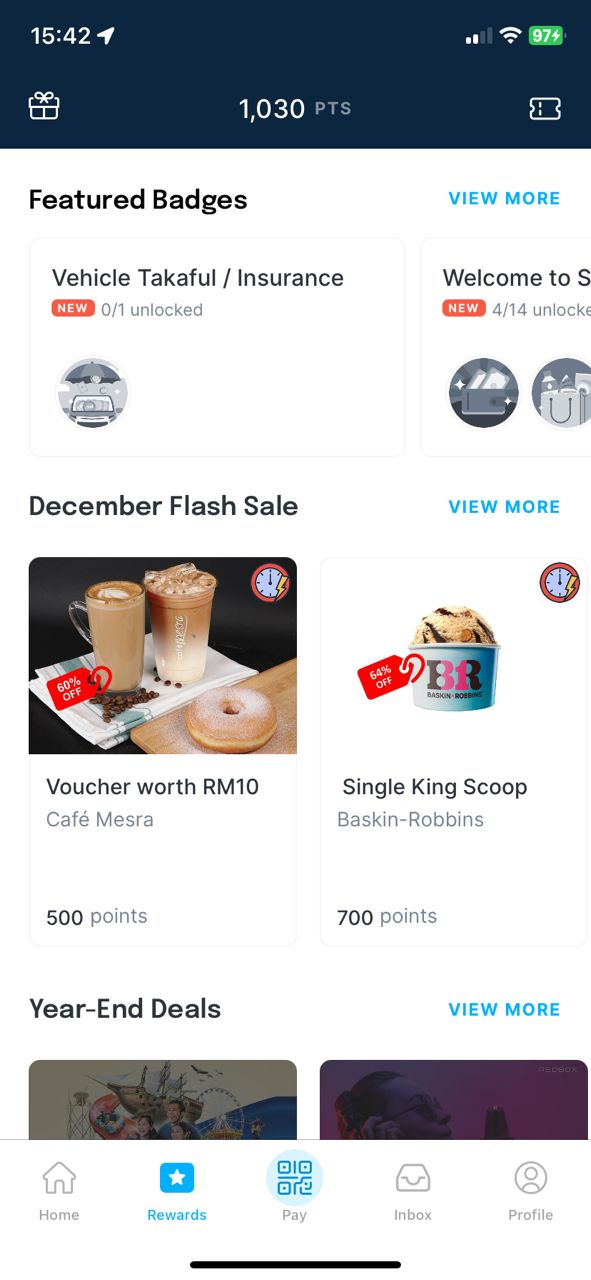
\includegraphics[width=0.35\linewidth]{mainmatter/images/gami1.jpg}
    \caption{Gamification Elements in Setel}
    \caption*{\textit{Screenshot of Rewards page in Setel [Setel Ventures Sdn. Bhd., 2023]}}
    \label{fig:myfig5}
\end{figure}
Figure 2.3 illustrates the gamified rewards page of the Setel mobile application, which is a comprehensive platform designed for the Malaysian audience, offering services such as fuel, parking, EV charging, eWallet, and more. This page utilizes gamification to prominently display users' earned points, promoting engagement by transforming routine transactions into chances to earn rewards. Users are motivated to actively engage in Setel's products, earning points that can be redeemed for practical vouchers in various categories such as food, fashion, and entertainment. The implementation of gamified design in Malaysia aims to provide an engaging and captivating experience for users. By using the principles of incentive and achievement, this design strategy fosters user loyalty. Additionally, it offers real and appealing rewards to further enhance user engagement.

\subsection{Technology Growth in Online Community}
Within the context of online communities, the profound impact of technology is obvious as it allows individuals to connect, exchange information, and engage with one another regardless of their physical location. The increasing availability of cell phones, high-speed internet, and easily accessible digital gadgets has facilitated the decentralization of membership in these communities, resulting in their increased accessibility and popularity. With the advancement of technology, online platforms have become more complex and engaging, providing a wide range of ways for people to express themselves and work together. \\

\textcite{leger21} underlines the unique features of sites such as Twitch and Bandcamp within the music industry. Twitch's distinctive monetization system differentiates itself by enabling musicians to directly generate revenue from their audience via subscriptions and virtual gifts. This promotes a more immediate and mutually beneficial connection between creators and fans, hence improving financial viability. On the other hand, Bandcamp's emphasis on selling albums and merchandise, rather than streaming, corresponds with evolving patterns of fan interaction, offering more concrete methods for audiences to show their support for their preferred artists. \\

Users actively interact with these platforms through various methods utilizing functionalities such as Twitch's real-time broadcasting or Bandcamp's direct sales approach. Nevertheless, difficulties remain, specifically in the realm of copyright concerns. These problems highlight the intricate nature that platforms encounter when trying to strike a balance between providing fair compensation for artists and safeguarding intellectual property rights \parencite{leger21}. Within the constantly changing digital environment, the integration of AI and machine learning is improving user experiences by providing personalized content recommendations and addressing security and privacy issues. With the advancement of technology, online communities are ready for further innovation, offering thrilling opportunities for individuals to interact, collaborate, and establish communities in the digital world.

\section{Music Discovery}
\subsection{Music Genre Diversity}
The concept of an extensive variety of genres in the process of discovering music has seen significant growth throughout recent years, driven by user-focused observations and developments in recommender systems. \textcite{robinson20} clarify the complex and varied aspects of diversity in music recommendation lists, underscoring the significance of integrating both internal and external diversity. Internal diversity, in this context, pertains to the assortment of subgenres and styles within a specific genre, whereas external diversity incorporates recommendations from entirely separate genres. These subtle and precise categories have fundamentally changed the way music enthusiasts explore and value varied musical landscapes. \\

In current recommender systems, measures such as variety, creativity, and randomness have become essential in addition to accuracy. When utilized in music discovery systems, these measures have a crucial impact in promoting genre exploration and expanding listeners' musical horizons. Diversity, as per the definition provided by \textcite{robinson20}, extends beyond the mere inclusion of random music. It encompasses the goal of achieving a well-proportioned representation of various genres and subgenres within recommendation lists. The presence of variety in music drives users to explore unfamiliar and unexplored musical categories, while randomness adds an element of pleasant unexpectedness, allowing listeners to come across genres they may not have encountered otherwise. \\

By utilizing user-centric information and metrics, modern music discovery services employ algorithms and curated playlists to direct listeners toward a wider range of genres. Through the integration of diverse elements from both internal and external sources, these platforms provide customized experiences that surpass the limitations of specific genres, promoting a wider musical exploration for users. Despite these circumstances, the recognition and enjoyment of many musical genres not only demonstrate the progress of technology but also highlight the influence of recommender systems in creatively influencing our musical preferences and tastes.

\subsubsection{Underrepresented Genres}
Traditional and local pop music, which is strongly influenced by tradition, frequently encounter difficulties in establishing a presence within popular music that appeals to a wider audience. However, online platforms have created an opportunity for enthusiasts to interact, exchange, and celebrate these genres. Online communities have arisen, attracting enthusiasts and musicians who are passionate about preserving and developing traditional music genres. Within these digital platforms, traditional and regional pop music genres receive acknowledgment and active involvement from an avid group of enthusiasts. \\

Digital platforms have a larger impact that goes beyond the establishment of genres. They facilitate the creation of music communities, surpassing geographical limitations and enabling persons with similar interests to unite. According to \textcite{silahudin19}, social media and online forums offer an environment for conversations, music sharing, and cooperation between musicians and their supporters. These groups not only cultivate admiration for underrepresented genres but also promote the production of novel music that combines traditional aspects with modern influences. \\

Eventually, the less popular music genres in the Malaysian music industry are discovering their expression and following the impact of digital platforms and online communities, as highlighted by \textcite{silahudin19}. These platforms facilitate the creation of genres such as traditional and regional pop music and promote the development of enthusiastic music communities. Thus, the music scene in Malaysia has grown in variety and comprehensive, preserving traditional practices while embracing originality and experimentation. \pagebreak

\subsection{Music Streaming Services Platforms}
Within the era of streaming, the process of discovering music has evolved and been shaped by both subjective experiences and social divisions based on socioeconomic status. \textcite{ellis20} explores the concept of "phenomenological moment" in the context of music discovery. He highlights the significant role these moments play in influencing individuals' interpretations and understandings of music. Music streaming platforms have emerged as a means of facilitating such experiences, allowing users to delve into a wide range of musical genres and artists that are customized to their preferences. These systems employ recommendation algorithms to enable users to find new music that connects with them, hence boosting the experiential aspects of music exploration. \\

In addition, users have progressively turned to music streaming sites as a method of storing and organizing their playlists \parencite{ellis20}. This method enables individuals to establish meaningful relationships with music over time, forming personal stories and connections with the songs they choose. Playlists surpass being simply collections of songs; they reflect an individual's musical journey and ever-changing preferences. This phenomenon highlights the fact that music streaming platforms not only make it easier to discover new music but also allow users to actively define their musical preferences and tastes. \\

\textcite{webster19} also explores the impact of music streaming platforms on individual preferences for music and the differentiation of cultural identities. These platforms have equalized access to music, erasing social class distinctions and enabling individuals from various backgrounds to explore and appreciate a wide variety of genres. Streaming services break common perceptions of modern and popular music by promoting user exploration free from the limitations of traditional class-based musical classifications. Music streaming platforms have played a significant role in creating a more inclusive and diversified music scene, prioritizing individual preferences over social class distinctions. \pagebreak

\subsubsection{Apple Music}
\begin{figure}[h]
    \centering
    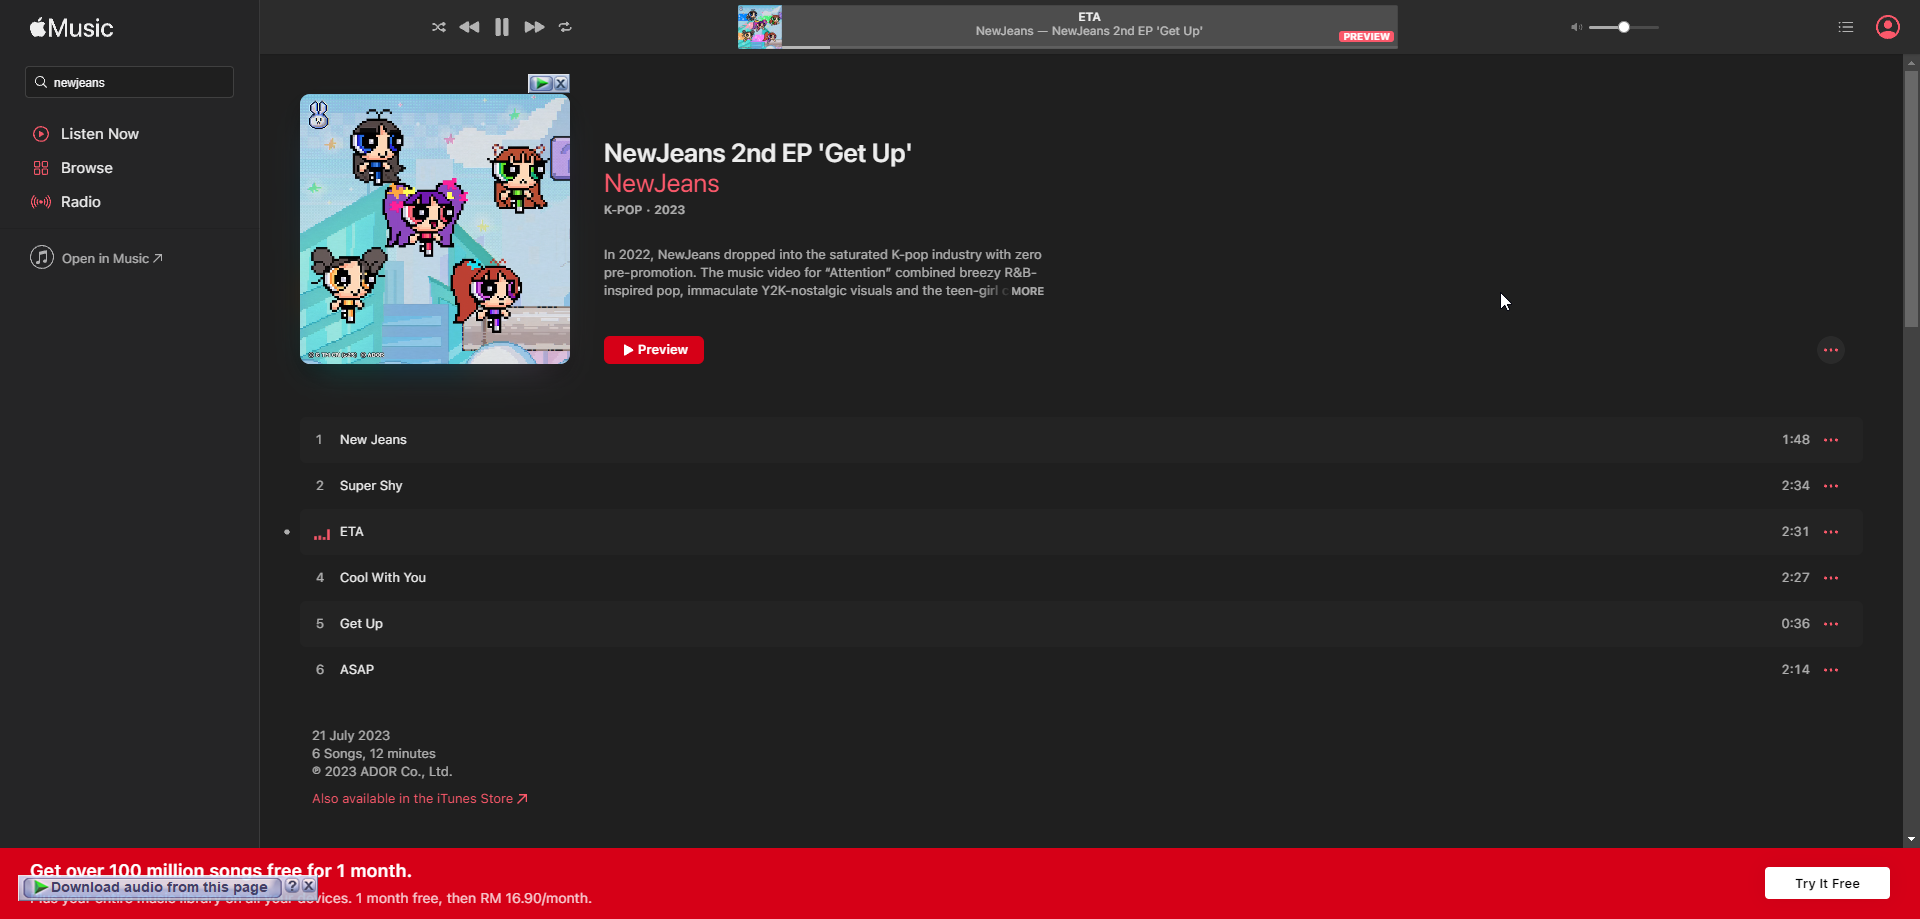
\includegraphics[width=1.0\linewidth]{mainmatter/images/musicplat1.png}
    \caption{Web Player for Apple Music}
    \caption*{\textit{Web Player Interface for Apple Music [Apple Inc., 2023]}}
    \label{fig:myfig6}
\end{figure}
Apple Music is a subscription-based music streaming service offered by Apple Inc. It provides users with access to a wide database of songs, albums, and playlists from various artists and genres. With features like personalized suggestions, curated playlists, and the opportunity to create your playlists, Apple Music offers a seamless and interactive music listening experience. Users can also download music for offline listening and enjoy exclusive content like music videos and artist interviews. It's available across numerous Apple devices and platforms, making it a simple alternative for people heavily ingrained in the Apple ecosystem. \pagebreak

\subsubsection{Spotify}
\begin{figure}[h]
    \centering
    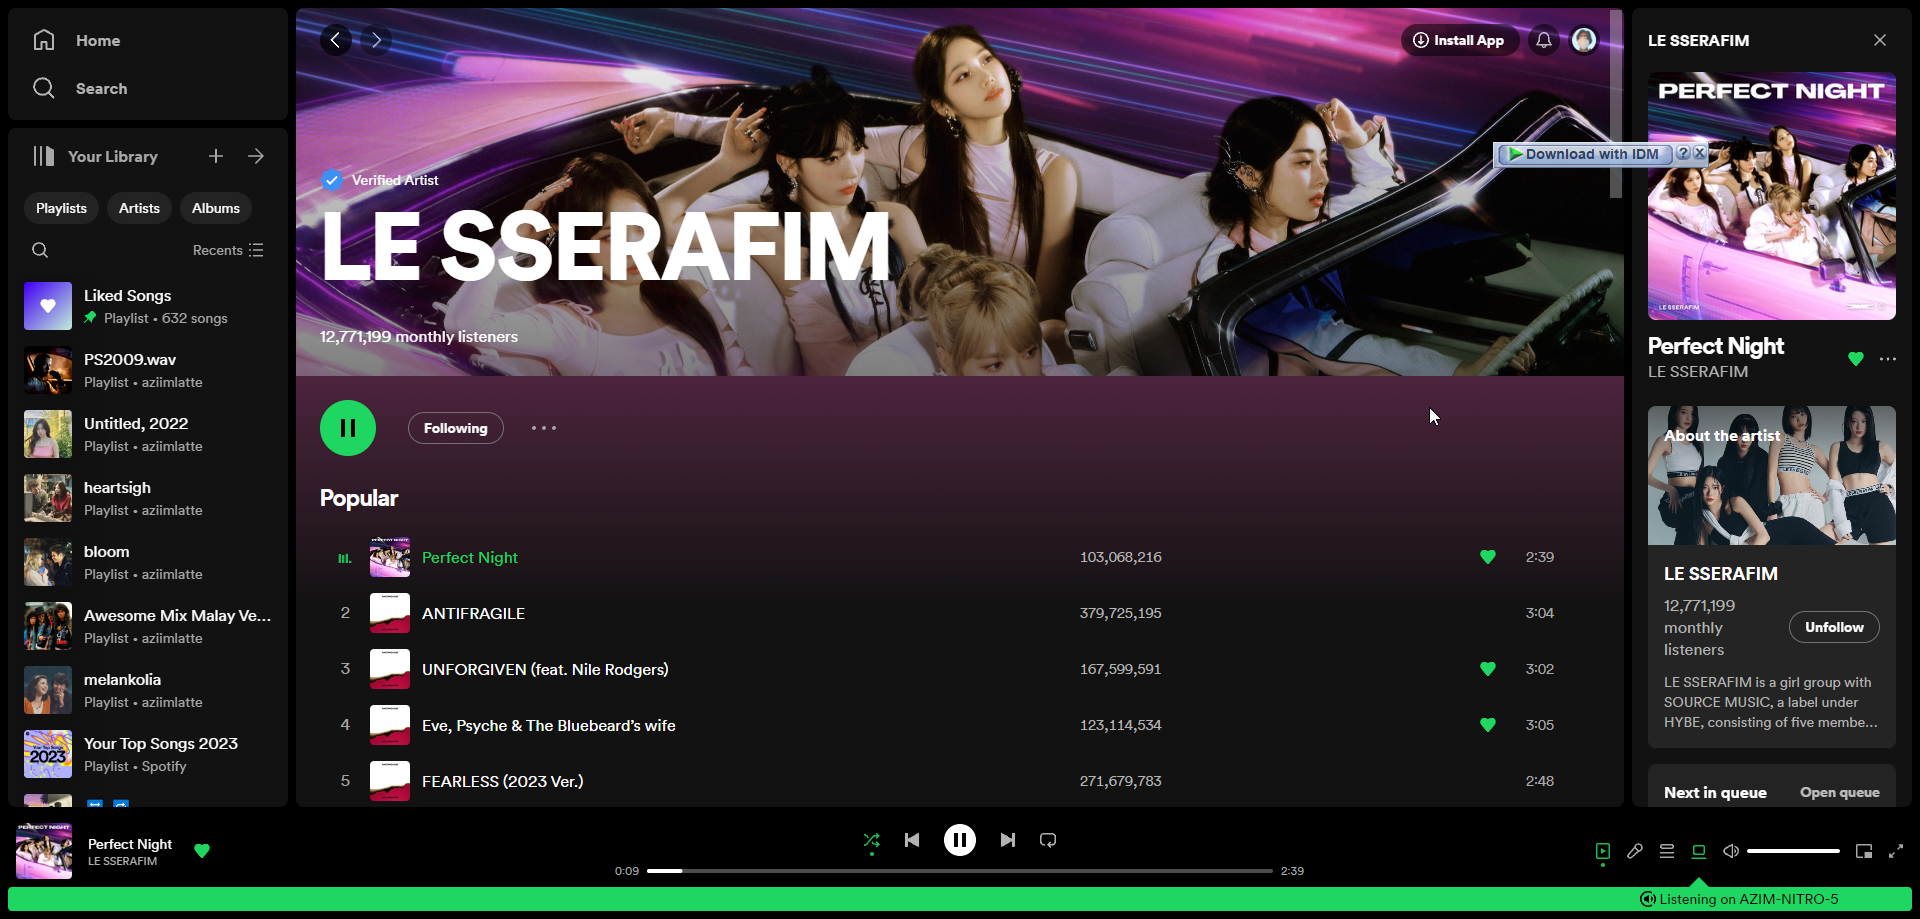
\includegraphics[width=1.0\linewidth]{mainmatter/images/musicplat2.png}
    \caption{Web Player for Spotify}
    \caption*{\textit{Web Player Interface for Spotify [Spotify Technology S.A., 2023]}}
    \label{fig:myfig7}
\end{figure}
Spotify is a popular music streaming platform that offers a wide catalog of songs, albums, and playlists from across the world. With both free and premium subscription options, it helps users discover, play, and share music effortlessly across numerous devices. Spotify's notable features include tailored playlists like Discover Weekly and Release Radar, as well as collaborative playlists, podcast streaming, and a social component that lets users follow friends and artists. It's known for its user-friendly interface, cross-platform compatibility, and a large range of music genres and content, making it a go-to pick for music enthusiasts searching for a diverse and accessible streaming experience. \pagebreak

\subsubsection{YouTube Music}
\begin{figure}[h]
    \centering
    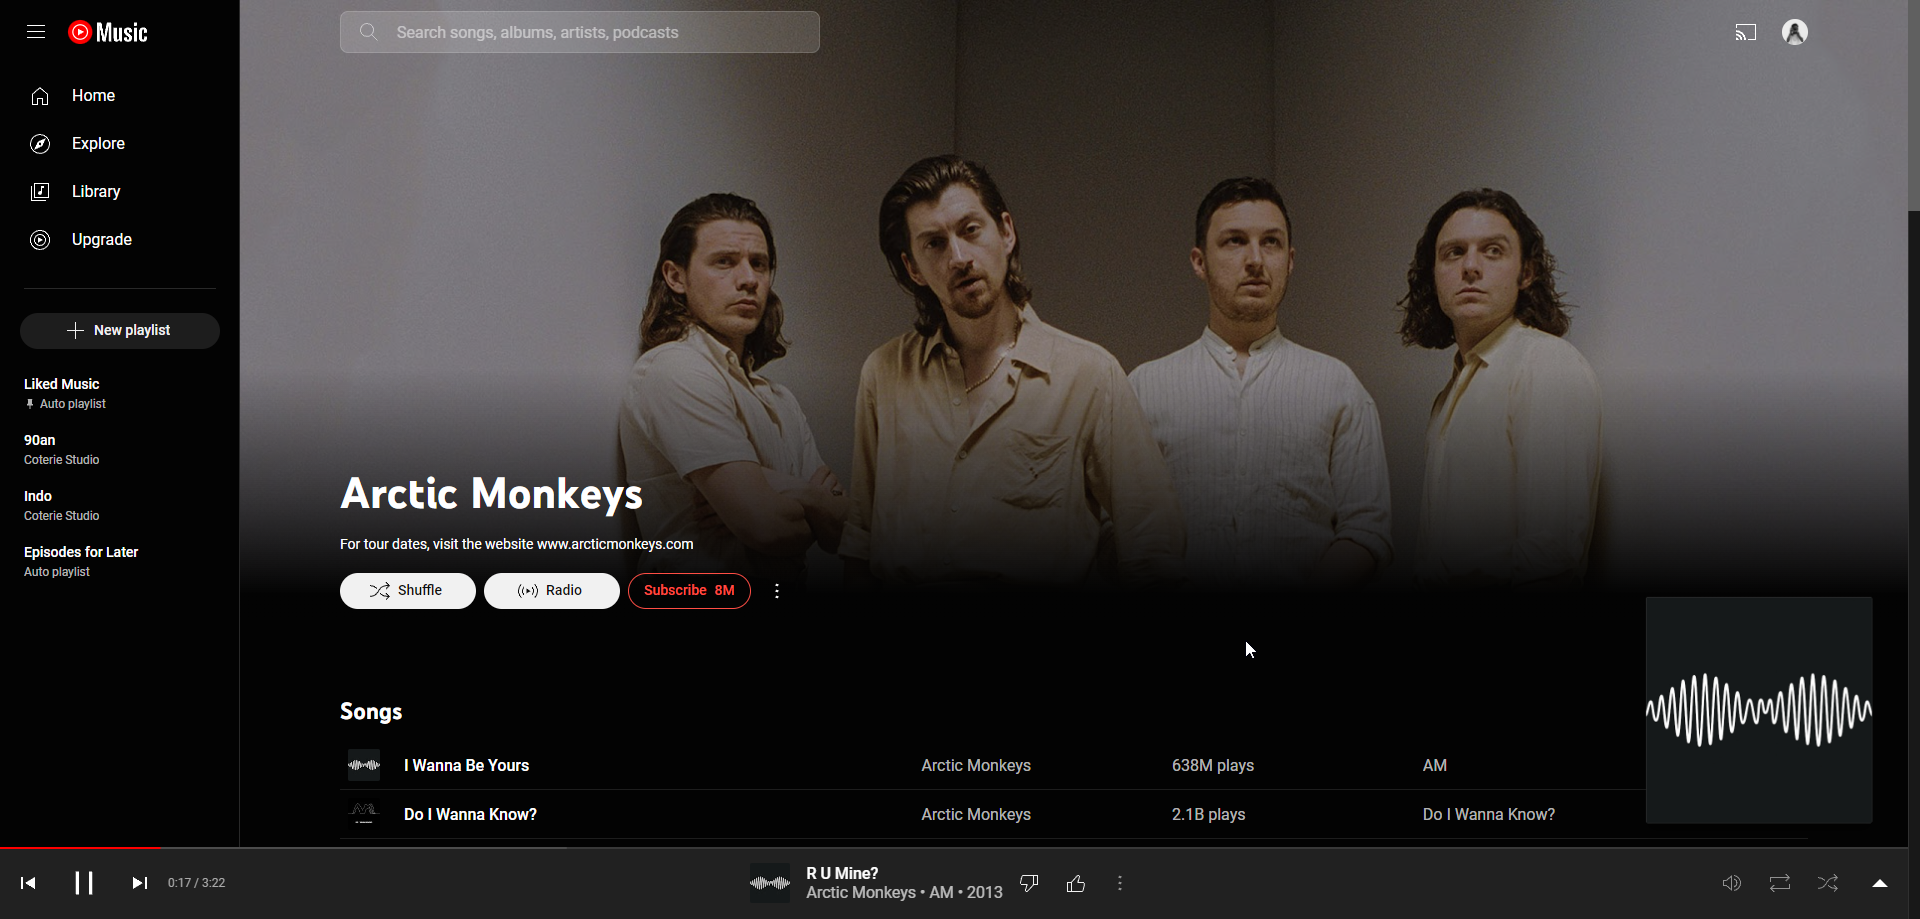
\includegraphics[width=1.0\linewidth]{mainmatter/images/musicplat3.png}
    \caption{Web Player for YouTube Music}
    \caption*{\textit{Web Player Interface for YouTube Music [YouTube and Google, 2023]}}
    \label{fig:myfig8}
\end{figure}
YouTube Music is a music streaming service provided by YouTube, specifically created to provide users access to an extensive collection of songs, music videos, and live performances. Within the broader YouTube ecosystem, this platform provides customized playlists, suggestions, and the option to discover music based on genre, artist, or mood. YouTube Music offers features such as offline downloading and background listening, making it a comfortable option for both free and paid members. YouTube Music appeals to a diverse audience of music lovers by offering a distinctive combination of authorized songs, content created by users, and music videos. This makes it a preferred option for individuals who appreciate visual elements in addition to their music. \pagebreak

\subsection{User Music Behavior}
The emergence of music streaming platforms and advanced recommendation algorithms has led to a significant transformation in user music behavior for music discovery. Conventional methods of exploring music, like radio broadcasts and physical record stores, have been replaced by more individualized and interactive techniques. This transition is consistent with the discoveries made by \textcite{liang22}, who investigated the progression of users' musical preferences over time. The significance of tailored forcing in genre exploration recommenders, emphasizes the function of exploration-oriented systems in fulfilling users' desires for novelty and diversity. \\

Moreover, the research conducted by \textcite{perera20} highlights the difficulties encountered by music recommendation systems in the current digital environment. These issues encompass a variety of brief song durations, huge music collections, and an excess of song recommendations. To address these problems, contemporary music recommendation systems have transitioned towards offering consumers personalized and varied recommendations, in line with the changing interests of users who desire a wider range of musical experiences. \\

Modern users need recommendations that not only align with their current interests but also promote exploration and discovery of new genres and artists, while also valuing certain views. This trend is especially apparent among users with greater musical expertise, who demonstrate more consistent tastes and a wider range of listening behaviors. Modern music discovery platforms place a high value on personalization, social engagement, and genre diversity to meet the changing interests and preferences of their users. This results in a more engaging and interactive music discovery experience. \pagebreak

\subsection{Music Promotion Strategies}
\subsubsection{Digital Marketing}
Music promotion has experienced an important shift in the current era of technology, with digital marketing emerging as a crucial element for both musicians and record companies. The proper utilization of online platforms can determine an artist's success in the fiercely competitive music industry. According to \textcite{haynes18}, social media enables direct interaction with the audience, which is a crucial aspect of promoting digital music. Nevertheless, their research also underscores the limitations of social media in accessing new audiences. \\

Digital marketing involves using several platforms to effectively target a wide demographic. Social media networks like Instagram, Facebook, and Twitter have a crucial impact. Artists and labels ought to consistently keep dynamic profiles, interact with fans, and regularly release captivating stuff. Musicians utilize social media channels to communicate with their audience, yet these platforms may have limitations in terms of reaching new audiences \parencite{haynes18}. This emphasizes the significance of expanding promotional techniques. \\

Developing and distributing captivating content is essential in the promotion of digital music. In addition to releasing music, artists can give exclusive insights into their creative process, music videos, and live performances. Employing visual media like YouTube and TikTok can also produce favorable outcomes. \textcite{basaran22} highlight the importance of customizing digital material and its influence on consumer happiness in the era of digital entertainment. In addition, they analyze the impact of social media on digital marketing, highlighting the fact that having a strong online presence does not always result in financial success for musicians. \\

Effective music promotion in the current digital context heavily relies on the implementation of digital marketing methods. To advance their music career, artists and labels should utilize social media, email marketing, and other content forms to engage with their audience, expand their influence, and eventually propel their music careers. By adopting these strategies and acknowledging their limitations, musicians can distinguish themselves in a saturated market and develop a loyal following, as evidenced by the studies conducted by \textcite{haynes18,basaran22}.

\subsubsection{Fan Engagement}
Interactive creation of content is a highly successful method for engaging fans. This includes live streaming sessions, question and answer sessions, and exclusive insights into the artist's personal life. This type of content cultivates a feeling of closeness and relationship between the artist and the fans. \textcite{edlom21} argue that fans actively participate in the creation of value within music brand communities by establishing emotional bonds and aligning their values with those of the artists. \textcite{lee20} explore participatory fandom, which emphasizes the active role of fans in shaping music promotion and exercising influence on commercial music services. \\

Personalization plays a crucial role in promoting fan involvement. Artists and labels can utilize email marketing and social media platforms to establish direct communication with their fans. This allows them to personalize the content by addressing fans by their names and personalizing it to their interests. Delivering customized messages for important occasions such as birthdays or album celebrations, expresses gratitude and strengthens the bond between the artist and their fans. Customized communication creates a sense of appreciation among followers and motivates them to maintain their loyalty and support. This is consistent with the dynamics of fan networks and their interactions with artists in a digital context, as explored by \textcite{edlom21}. \\

Establishing a digital community focused on the artist's music is an effective approach to engage fans. Artists can establish fan clubs, forums, or exclusive groups on popular platforms such as Facebook or Discord. These spaces provide opportunities for fans to interact, express their enthusiasm for the music, and participate in conversations. The artist's active engagement in these groups develops a feeling of belonging and guarantees that fans receive sufficient details about upcoming releases and activities. \textcite{lee20} found that the connection between music enthusiasts and commercial music platforms is shaped by participatory fandom, highlighting the significance of fan involvement in music promotion. \\

Fan engagement is more than an aspect of music promotion; rather, it serves as the core foundation upon which successful music careers are established. Strategies such as creating interactive material, engaging in personalized contact, and promoting a sense of community are crucial for establishing deep connections with followers. Both \textcite{edlom21} and \textcite{lee20} emphasize that these connections can result in increased audience pleasure, collaborative value creation, and sustained support for the artist's work. By placing audience involvement as a top priority, musicians and record labels can establish a durable and successful music ecosystem in the digital age.

\section{Mobile Application}
A mobile application, usually referred to as a mobile app or just an app, is a software program designed specifically to run on mobile devices such as smartphones, tablets, or smartwatches \parencite{ramdurai21}. These applications provide a broad range of functions, including basic operations like weather checking and more complex objectives like financial management. These applications can be accessed through platforms such as Apple's App Store or Google Play Store. They make use of touchscreen interfaces and device-specific technologies, such as cameras and GPS, to provide customized and interactive experiences. Mobile app development involves the process of writing, testing, and optimizing applications for different mobile platforms such as iOS and Android. This is done using programming languages like Swift, Objective-C, Java, and Kotlin. User experience (UX) and user interface (UI) design are essential elements that guarantee both functionality and visual appeal. In the current era of digitalization, mobile applications have become an essential component of everyday life, providing comfort, entertainment, and productivity tools readily accessible.

\subsection{Type of Mobile Application}
Mobile applications can be classified into three primary categories: native applications, web-based applications, and hybrid applications \parencite{syeed21}. Native apps are designed for a specific platform and are created using the programming languages native to iOS or Android. They provide excellent performance and smooth user experiences, while also allowing access to capabilities exclusive to the device. On the other hand, web-based applications can be accessible via mobile web browsers, ensuring compatibility across different platforms, eliminating the need for installation, and enabling easier development through the use of common web technologies. Hybrid applications combine components from both native and online apps, using web technologies enclosed within a native container to facilitate development across many platforms, partial utilization of native functionalities, and dissemination through app stores. The selection among these categories is dependent upon aspects such as performance requirements, target demographic, and development resources, with each method having its unique variety of benefits and limitations.

\begin{figure}[h]
    \centering
    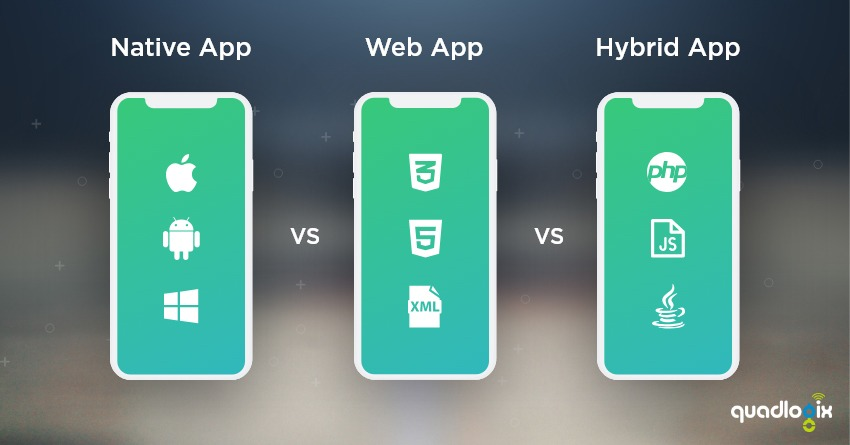
\includegraphics[width=1.0\linewidth]{mainmatter/images/typeapp.jpg}
    \caption{Type of Mobile Application}
    \caption*{\textit{NATIVE VS WEB VS HYBRID MOBILE APPS [QuadLogix, 2019]}}
    \caption*{https://www.quadlogix.com/blog/web-vs-native-vs-hybrid-mobile-apps-the-right-way-for-enterprises/}
    \label{fig:myfig9}
\end{figure}

\subsubsection{Native Application}
A native application, as defined by \textcite{syeed21}, is a software program that is carefully created to work exclusively on a particular operating system, such as Android or iOS. This application is specifically designed to maximize the utilization of the built-in functionalities and capabilities of the intended platform. Native apps offer enhanced speed compared to cross-platform or web programs due to their strong integration with the operating system, utilization of platform-specific tools, and support for advanced features including gestures, notifications, and hardware functionality such as Bluetooth, NFC, sensors, and cameras. In Android development, the programming languages Java or Kotlin and the software Android Studio are used. On the other hand, iOS development makes use of either Objective-C or Swift, along with XCode. Native apps offer several benefits, including improved speed and efficiency, better use of resources, and the ability to provide a secure and engaging user experience. Nevertheless, there are certain disadvantages associated with this approach, such as the requirement for distinct development for each platform, increased development expenses, and proficiency in platform-specific programming languages.

\subsubsection{Web Application}
According to \textcite{syeed21}, web applications are websites that are created to imitate the look and behavior of responsive websites. These applications are created using HTML5, CSS, and JavaScript. They are designed to run on web browsers and can be installed by creating bookmarks on the corresponding pages. Web apps do not possess the same level of functionality and performance as native apps. Their development encompasses technologies such as HTML5, CSS, and JavaScript for the client side, as well as server-side technologies like PHP, Perl, Python, or Ruby. The benefits of web applications include their ability to be deployed on any platform, their minimum storage requirements on the device, and their simpler maintenance through automatic web-based updates. Nevertheless, there are certain disadvantages to consider. This approach cannot produce performance-focused apps like 3D games, has poor user interface customization, and performs poorly compared to native applications due to Web View limitations.

\subsubsection{Hybrid Application}
Hybrid applications, as explained by \textcite{syeed21}, are a combination of native and online applications, combining the advantages of each. These applications are offered via app stores and can take advantage of specific built-in functionalities while using HTML within a web browser for display. Hybrid apps, although they may seem and work like native apps, are online apps that run on a browser. This strategy expands the developer's scope to a wider audience, allowing for app distribution via app stores and facilitating the tracking of downloads. Several frameworks, including React Native, Flutter, Cordova, Ionic, and Xamarin, offer options for developing hybrid applications. The benefits of hybrid apps include accelerated and cost-effective development in comparison to native versions, the ability to maintain a single code base that updates simultaneously on targeted platforms, offline availability, and suitability for swiftly releasing a Minimum Viable Product (MVP). However, this approach has drawbacks like the inability to create performance-focused applications like 3D games, reduced performance compared to native applications due to Web View restrictions, and poor user interface customization.

\subsection{User Experience Design}
As stated by \textcite{olawole18}, User Experience (UX) design and Human-Computer Interaction (HCI) are essential components in the development of efficient and user-friendly digital interfaces. UX design aims to optimize the whole user experience during product interaction, incorporating factors such as usability, accessibility, and emotional reaction. Human-Computer Interaction (HCI) is a comprehensive discipline that explores the relationship between humans and computers, with a particular focus on designing and utilizing computer systems from a human-centric standpoint. \\

The objective of UX design is to develop interfaces that are user-friendly, visually appealing, and effective, guaranteeing seamless navigation and task completion for users \parencite{olawole18}. This entails performing user research, establishing user personas, and implementing design principles to steer the development process. Usability testing is an essential component of UX design, enabling designers to collect feedback and refine their designs based on actual user interactions. \\

Human-Computer Interaction (HCI) is a field that explores the scientific study of human-computer interaction and the development of innovative technologies that facilitate human-computer interaction. The field of study incorporates insights from several fields including psychology, cognitive science, and ergonomics to comprehend how people perceive, interpret, and react to digital interfaces. Human-Computer Interaction (HCI) spans the entirety of the user's experience, analyzing elements such as methods of input, mechanisms of feedback, and the general design of interactive systems \parencite{olawole18}. \\

The collaboration between UX design and HCI is crucial for developing digital interfaces that not only fulfill functional needs but also deliver a favorable and significant user experience. Practitioners in the domains of user research, psychology, and design approaches utilize a combination of knowledge to ensure that technology is not just usable but also fun and satisfying for users.

\subsection{Challenges of Mobile Application Development}
The process of developing mobile applications presents significant opportunities but also poses many problems. An important obstacle lies in the fragmentation among many mobile platforms, such as iOS and Android, each requiring different development methodologies. Developers frequently encounter the task of providing uniform functioning and user experience across a wide range of devices, screen sizes, and operating systems \parencite{syeed21}. To bridge this gap, it is necessary to have a thorough comprehension of the complexities of each platform and conduct careful testing to ensure the best possible performance. \\

Mobile app development is significantly challenged by security considerations. Given that mobile applications manage sensitive user data, it is crucial to prioritize the implementation of strong security mechanisms \parencite{wambua23}. Developers must incorporate encryption, secure data storage, and authentication procedures to safeguard user information from potential risks like as data breaches and unauthorized access. Keeping up with advancing security requirements and mitigating vulnerabilities requires ongoing attention throughout the whole development process. \\

The rapid advancement of technology presents the difficulty of keeping up-to-date with the most recent trends and upgrades. Mobile platforms, programming languages, and development frameworks undergo regular modifications, necessitating developers to adjust and take advantage of new capabilities and improvements \parencite{syeed21}. Staying competitive in the ever-changing field of mobile app development requires dedicating time and effort to continuously learn and improve. \\

Finally, meeting user expectations for smooth and instinctive experiences poses a continuous challenge. As users become more knowledgeable, developers must consider usability, responsiveness, and overall user pleasure. As explained by \textcite{olawole18}, achieving a harmonious balance between usefulness, a visually appealing and intuitive design, and achieving performance standards is a complex task that necessitates a deep comprehension of user behavior and preferences.

\subsection{Features of Mobile Application}
\subsubsection{Profile Creation}
\begin{figure}[h]
    \centering
    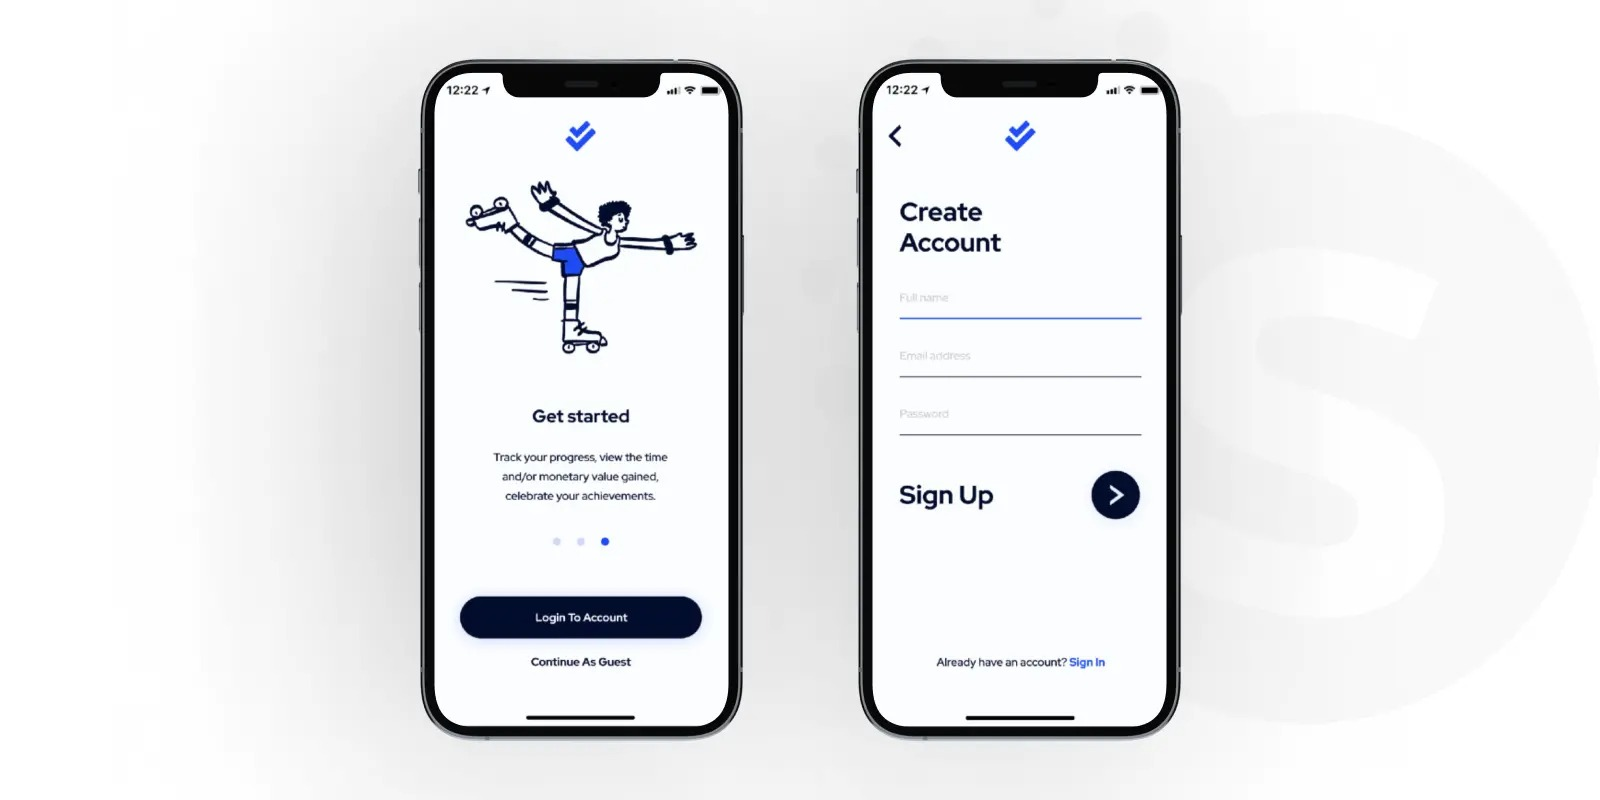
\includegraphics[width=0.9\linewidth]{mainmatter/images/userprofile.jpg}
    \caption{Registration Page User Interface (UI) Design}
    \caption*{\textit{Registration form UX [Softermii, 2022]}}
    \caption*{https://www.softermii.com/blog/19-ux-design-tips-for-shopping-app-with-examples}
    \label{fig:myfig10}
\end{figure}
The user profile creation feature in a mobile application plays a fundamental role in establishing a deeper connection between users and the app's ecosystem. It enables users to establish their distinct digital identity, hence increasing their entire experience. Throughout the profile creation procedure, users commonly provide essential details such as their name, email address, and password, which are securely maintained for account management and communication. Establishing this foundation is crucial for building confidence and guaranteeing the protection of data. \\

In addition to providing fundamental details, the process of creating a user profile frequently presents possibilities for customization. Users can post a profile photo, which enhances the visual appeal of their account and promotes a sense of familiarity and identification among the app's community. Moreover, the ability to customize settings and preferences empowers users to precisely adjust their experience. Users can customize notifications, select theme colors, and establish preferences for content recommendations, resulting in the app seeming like a personalized extension of their digital existence. \\

\textcite{abdulrahman22} highlight the increasing importance of creating a mobile application that includes a function for users to create profiles. This functionality enables users to create and control their profiles within the application, so improving their capacity to customize their experience and interact with the platform according to their preferences and experiences. Incorporating such a characteristic aligns with the insights made by \textcite{weichbroth20} regarding the user-friendliness of mobile applications. \\

\textcite{weichbroth20} also highlights the significance of guaranteeing an efficient and accessible procedure for creating user profiles. To tackle this usability element, mobile application developers must give priority to the creation of an intuitive and easily navigable user interface. It is important to provide concise instructions and a streamlined process to enable users to easily finish their profiles. Furthermore, it is vital to offer consumers the capability to effortlessly modify and update their profile details, allowing for adjustments in their preferences or conditions. \pagebreak

\subsubsection{Music Snippet Sharing}
\begin{figure}[h]
    \centering
    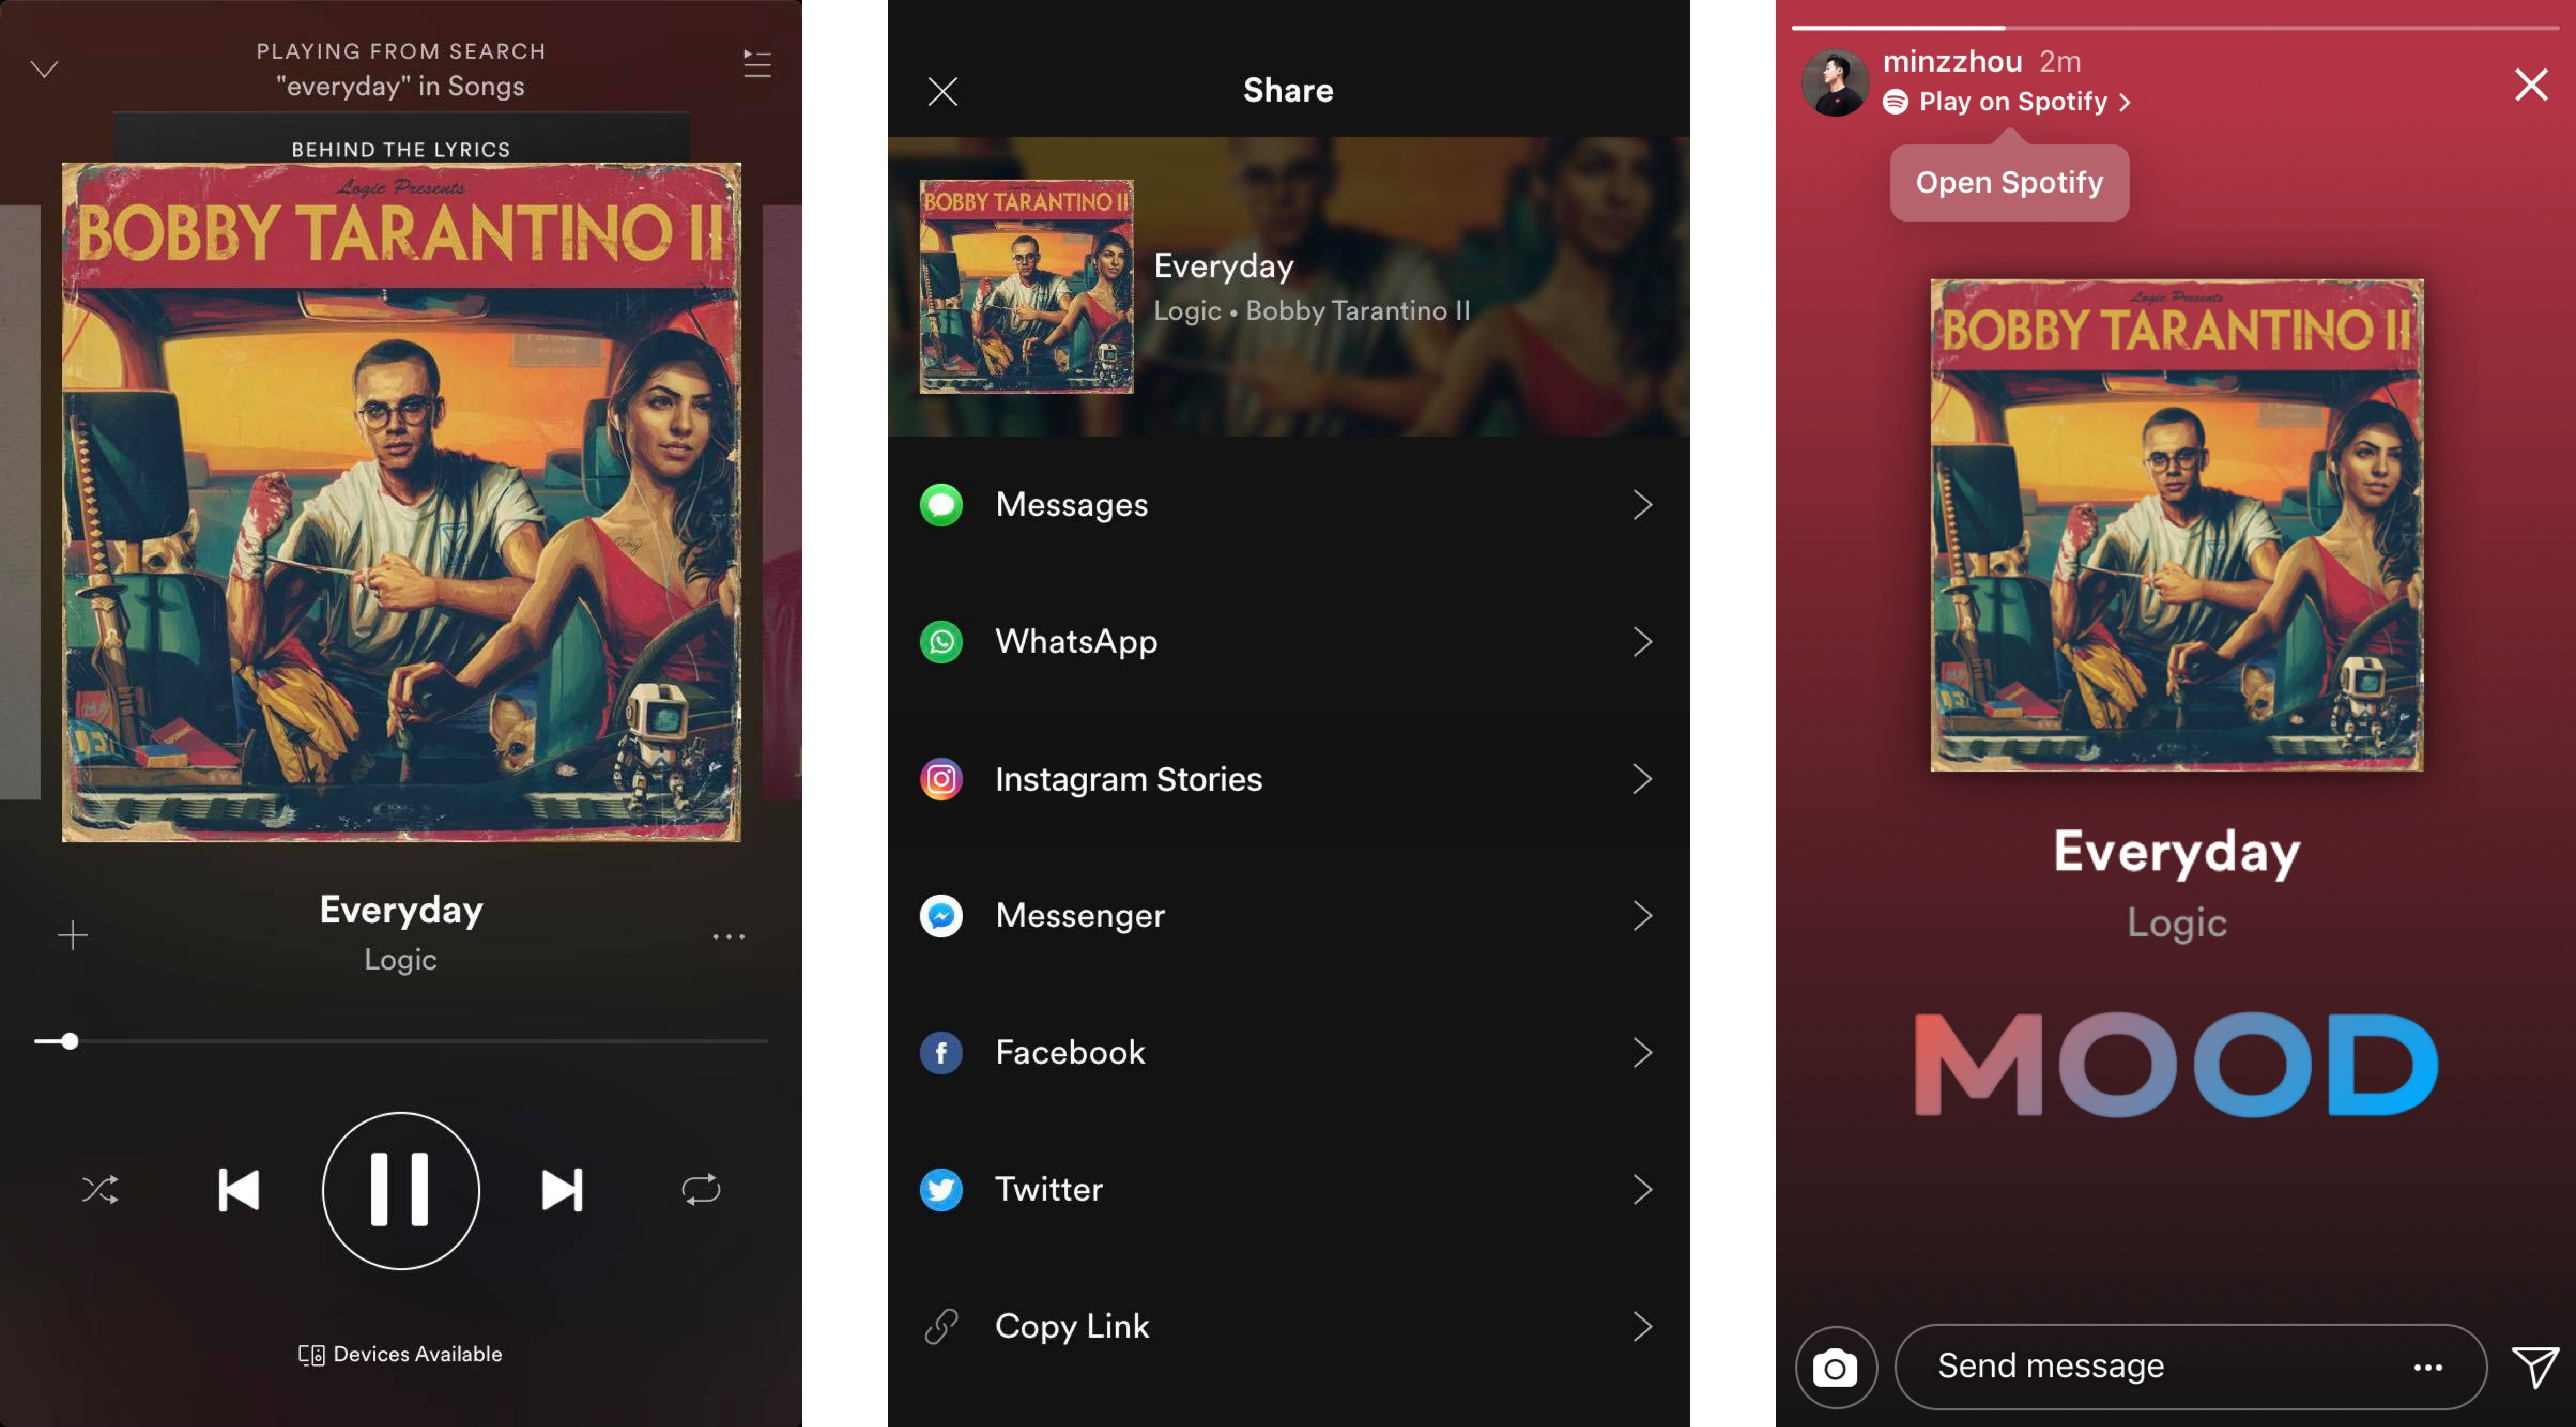
\includegraphics[width=1.0\linewidth]{mainmatter/images/musicshare.jpg}
    \caption{Spotify Sharing to Instagram Stories}
    \caption*{\textit{Instagram Adding Spotify Content-Sharing to Stories [Variety, 2018]}}
    \caption*{https://variety.com/2018/digital/news/instagram-stories-spotify-ar-video-chat-1202793586/}
    \label{fig:myfig11}
\end{figure}
The music snippet-sharing option in a mobile application is a versatile and captivating tool that enables users to share their preferred music moments with friends and followers. This functionality enables users to choose and distribute brief sections or "snippets" of songs, resulting in a customized and engaging musical encounter. It improves the social dimension of music consumption and encourages the exploration of music enjoyably and engagingly. \\

Music snippet sharing is a popular function in mobile applications, such as Apple Music, Spotify, and SoundCloud. Users can readily utilize this feature by picking music from their library or the streaming service's catalog and subsequently selecting a specific segment of the track to share. These snippets can be customized to capture the most engaging parts of the music, be it a catchy chorus, a memorable guitar riff, or a stunning vocal performance. After users generate these snippets, they may easily distribute them on other platforms, such as popular social media networks like Facebook and Twitter, messaging apps like WhatsApp, or within the application's social network. This function amplifies the process of finding new music, promotes interaction with others, and introduces a dynamic element to the overall user experience in these mobile applications that prioritize music. \\

The music snippet-sharing feature in mobile applications has surely transformed the way users connect with music and each other. Moreover, a recent study by \textcite{abdulrahman22} on user-generated content and reviews in mobile applications suggest a potential connection with music snippet sharing. The creation of a mobile application that encourages users to post reviews based on their experiences with a service suggests a bigger user-generated content feature. This bigger functionality might potentially involve the sharing of music snippets or related content within the program. By incorporating user-generated music elements alongside reviews, mobile apps may build a more comprehensive and engaging platform that caters to users' different interests and preferences. \\

From a usability aspect, \textcite{weichbroth20} underlines the significance of simplicity and intuitiveness in the sharing process. To make music snippet sharing effortless, mobile applications must prioritize an easy-to-navigate user interface with clear instructions and few actions required to share a snippet. Furthermore, offering users the opportunity to share snippets through numerous channels, such as social media or messaging apps, guarantees that users can effortlessly spread their favorite music moments and communicate with their friends and followers on their preferred platforms. \pagebreak

\subsubsection{Favourite/Bookmark}
\begin{figure}[h]
    \centering
    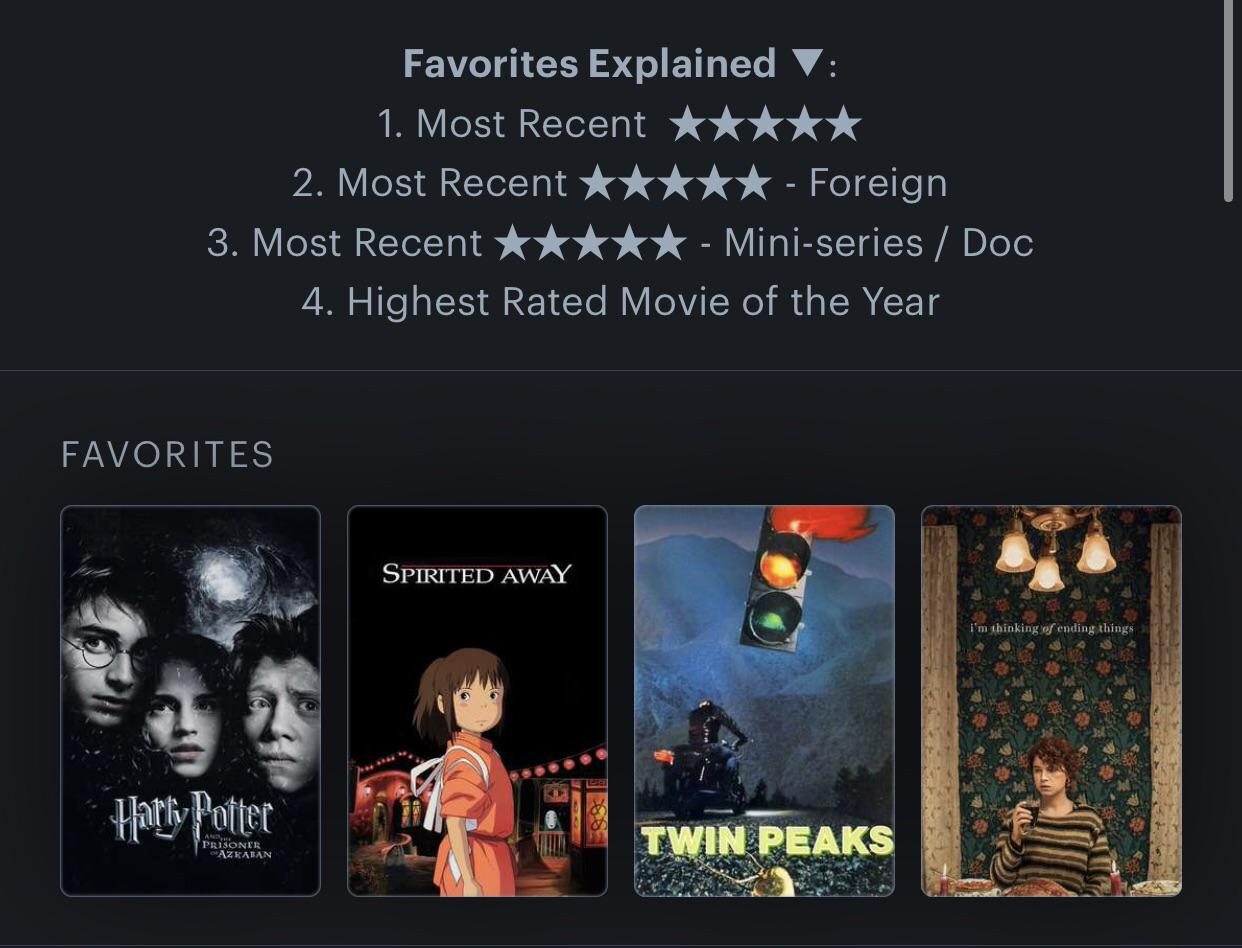
\includegraphics[width=0.8\linewidth]{mainmatter/images/favbookmark.jpg}
    \caption{Screenshot of Letterboxd Favourite/Bookmark Feature}
    \caption*{\textit{Letterboxd Favourite/Bookmark Feature [Reddit, 2020]}}
    \caption*{https://www.reddit.com/r/Letterboxd/comments/iyxsay/how-i-arrange-my-favorites-how-do-yall-arrange/}
    \label{fig:myfig12}
\end{figure}
The favorite or bookmark feature in a mobile application is an essential feature that empowers users to save and organize content that carries personal meaning or interest. Whether it's articles, movies, products, or any other type of digital material, this feature allows users to curate their digital collections for simple access and reference. By simply marking material as a favorite or bookmarking it, users may easily manage their digital life and increase their overall user experience. \\

Users can often access this function by clicking on a specific icon or option within the application, which subsequently saves the selected content to a personalized list. This list can be readily sorted and categorized, ensuring that users can quickly recover their saved things whenever they need them. Additionally, the favorite/bookmark feature sometimes provides opportunities to add notes or tags, further boosting information organization and retrieval. \\

The favorite or bookmark feature in a mobile application not only allows content management but also aligns with the findings of a recent study. \textcite{abdulrahman22} explore how mobile applications allow users to bookmark or save chosen material, essentially adding a functionality similar to a favorites or bookmark feature within the program. This shows the relevance of such features in appealing to user preferences and enabling content management. \\

From a usability standpoint, as noted by \textcite{weichbroth20}, it is crucial to ensure that the process of adding information to favorites or bookmarks is user-friendly. Mobile applications must offer an intuitive user experience that is easy to navigate, with clear instructions and few steps required to add material to favorites or bookmarks. Additionally, allowing users to modify and organize their favorites or bookmarks in a way that makes sense to them enhances the usability and customization of the function. \pagebreak

\subsubsection{Ratings or Reviews}
\begin{figure}[h]
    \centering
    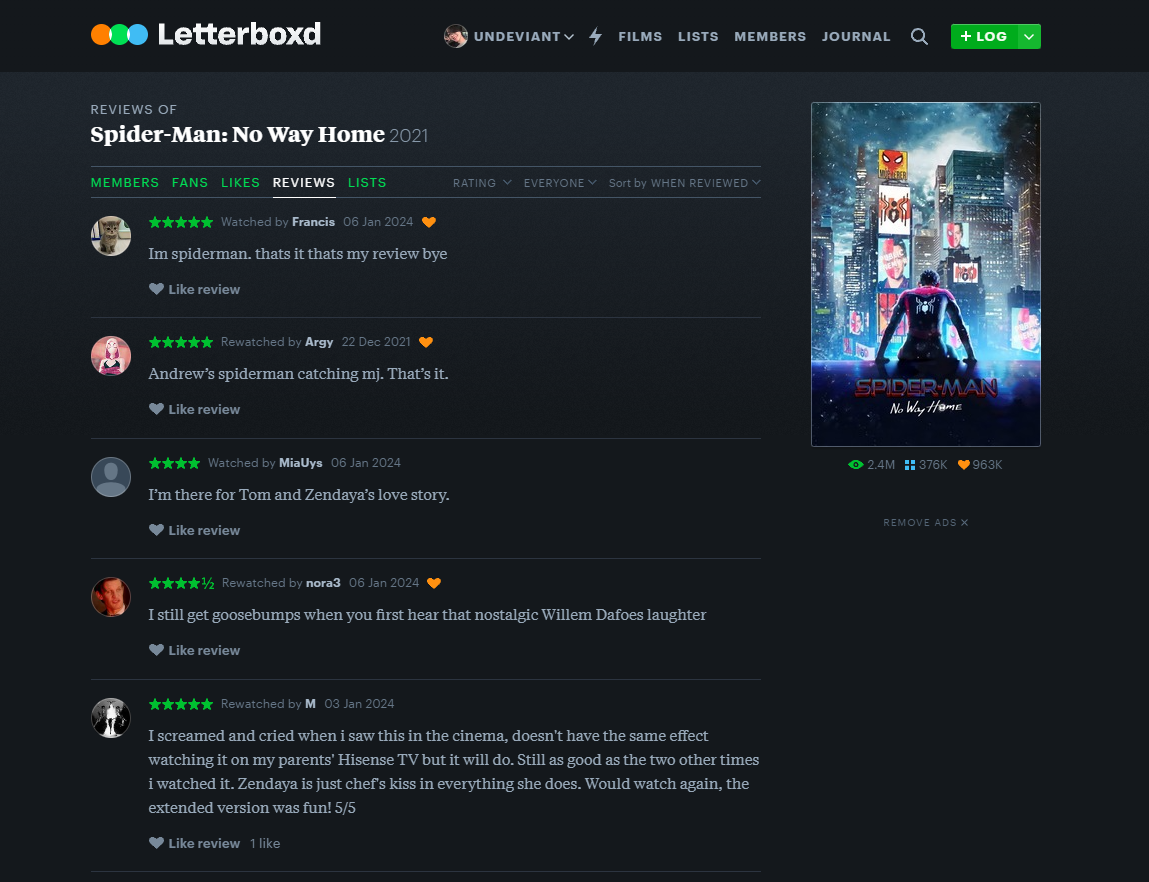
\includegraphics[width=0.8\linewidth]{mainmatter/images/ratingsreviews.png}
    \caption{Screenshot of Letterboxd Reviews Page}
    \caption*{\textit{Letterboxd Reviews Page [Letterboxd, 2024]}}
    \caption*{https://letterboxd.com/film/spider-man-no-way-home/reviews/by/added/}
    \label{fig:myfig13}
\end{figure}
The ratings and reviews functionality in a mobile application is an essential tool that enables users to provide feedback, interact with the app, and make informed decisions. Users can utilize this functionality to express their experiences, viewpoints, and evaluations of the app, products, services, or material offered within the application. Typically, it entails assigning a numerical rating and providing textual comments to articulate their opinions, resulting in a valuable collection of user-generated content. \\

Users can utilize the ratings and reviews functionality by accessing it through the application's interface, typically by browsing to a dedicated section or tapping on a specified icon. This feature offers prospective users or customers crucial information regarding the excellence and trustworthiness of the app or its offerings. Ratings, commonly depicted as star ratings or numerical scores, provide a concise and immediate visual indication of user contentment, whereas reviews offer detailed analysis and commentary that can assist individuals in making well-informed choices. \\

The ratings and reviews function in a mobile application is important from both a user-centric and usability standpoint. \textcite{abdulrahman22} emphasize the significance of genuine content evaluations and comments provided by users who have experienced a service. The focus on genuine user-generated evaluations and ratings underscores the crucial function this feature serves in aiding users to make well-informed choices. It guarantees that the feedback given is trustworthy and accurately represents genuine user experiences, enhancing the trustworthiness of the evaluated app or service. \\

According to \textcite{weichbroth20}, it is crucial to ensure that the rating and review process is user-friendly and easy to understand. The user interface should be created with maximum clarity, explicit instructions, and a simplified method to evaluate or review information, minimizing the number of steps required. Furthermore, enhancing the usability of this feature can be achieved by offering users the option to conveniently access and organize ratings or reviews according to their preferences, such as by date or by rating. Moreover, it is essential to uphold transparency and equity in the rating and review system, with clearly established criteria for determining a high or low rating. This guarantees that the feature maintains its reliability and worth for both consumers and developers. \pagebreak

\section{Reviews of Existing Mobile Application}
\subsection{Letterboxd}
\begin{figure} [h]
    \centering
    \begin{subfigure}{.3\linewidth}
      \centering
      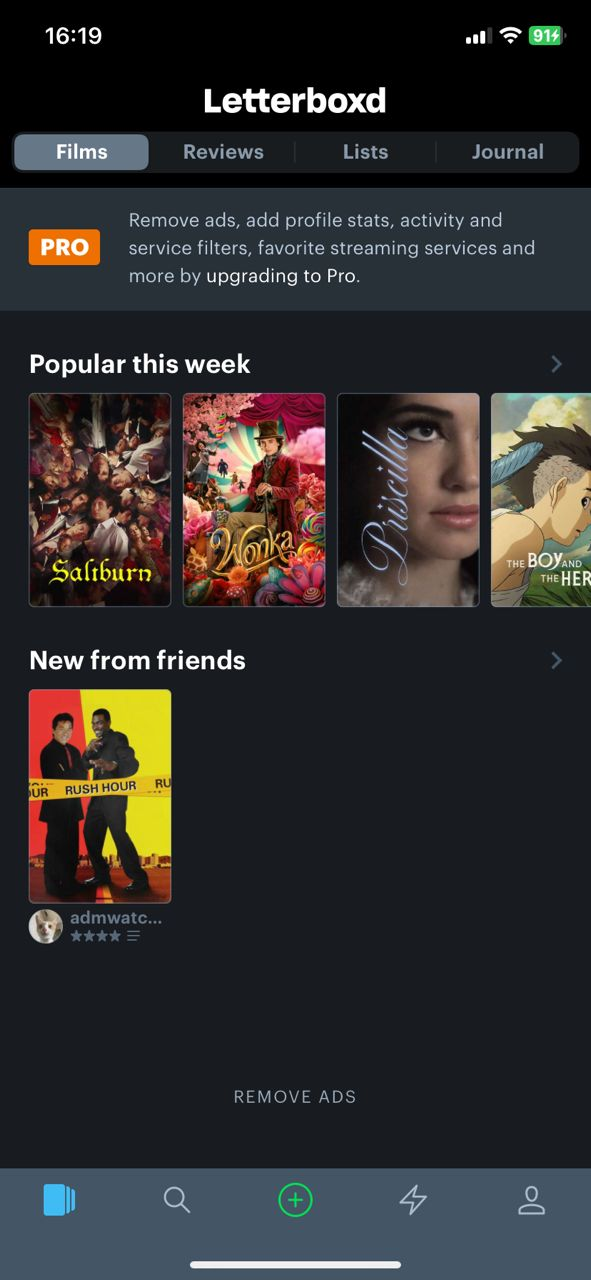
\includegraphics[width = \linewidth]{mainmatter/images/letterboxd1.jpg}
      \caption{Home Page}
      \label{fig:myfig14}
    \end{subfigure}%
    \hspace{1em}% Space between images A and B
    \begin{subfigure}{.3\linewidth}
      \centering
      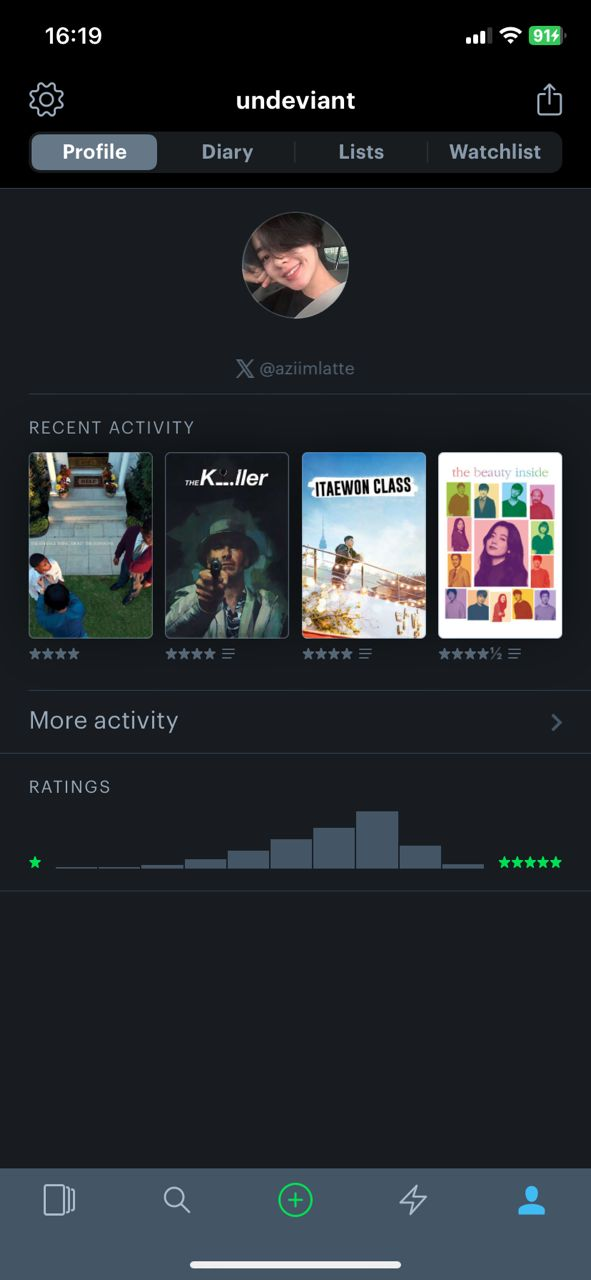
\includegraphics[width = \linewidth]{mainmatter/images/letterboxd2.jpg}
      \caption{User Profile}
      \label{fig:myfig15}
    \end{subfigure}%
    \hspace{1em}% Space between images B and C
    \begin{subfigure}{.3\linewidth}
      \centering
      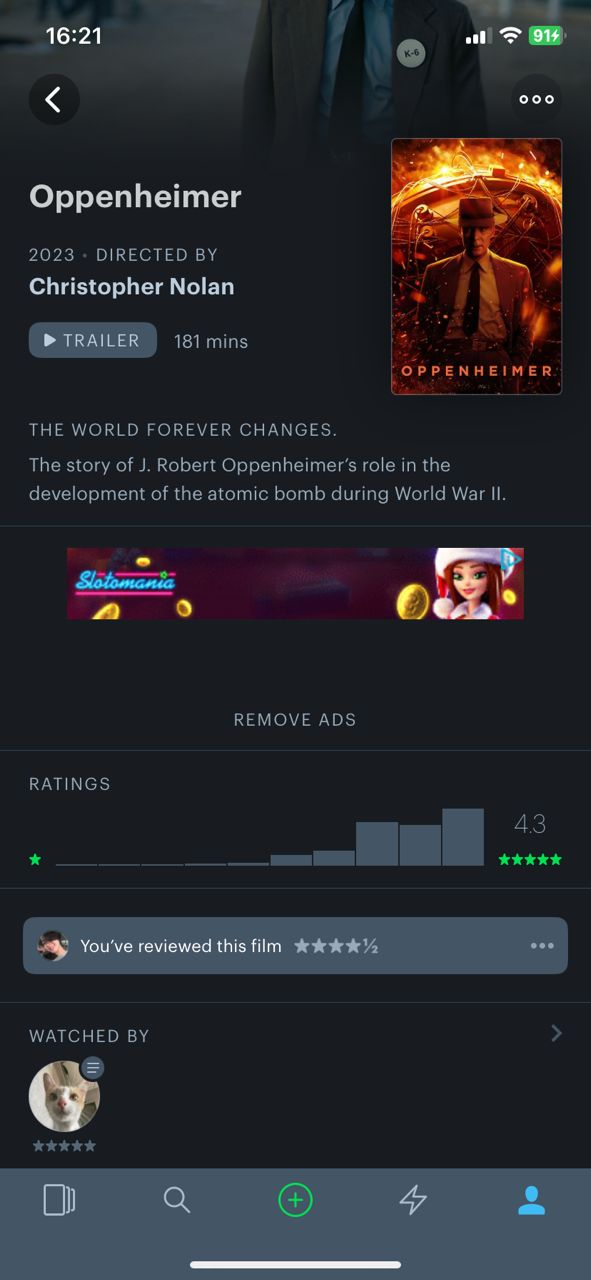
\includegraphics[width = \linewidth]{mainmatter/images/letterboxd3.jpg}
      \caption{Film Page}
      \label{fig:myfig16}
    \end{subfigure}
    \caption{Screenshots from Letterboxd Mobile Application}
    \caption*{\textit{Mobile Application Interface for Letterboxd [Letterboxd, 2024]}}
\end{figure}
Letterboxd is a widely-used mobile application designed for film enthusiasts, offering a platform for tracking, evaluating, and exploring films. The application enables users to establish and manage a customized film diary, where they can record films they have viewed, assign ratings, and write reviews. The UI is designed to be easily understandable and accessible to users, and it includes an extensive database of films, with comprehensive information such as the cast, crew, release date, and genre. In addition, Letterboxd promotes a feeling of community by enabling users to track one another, provide feedback on reviews, and exchange their cinematic encounters. The application is compatible with both Android and iOS platforms, ensuring its accessibility to a wide spectrum of users. \pagebreak
\begin{itemize}[\label{}]
    \item \textbf{Advantages} \\
    A vital feature of Letterboxd is its extensive film database, which allows users to effortlessly explore and find new films. The app's social component promotes engagement among film enthusiasts, creating a feeling of relationship and offering a platform for conversation on cinematic topics. The app's personalized cinema diary function serves as a great tool for users to thoroughly record their viewing history, hence facilitating recommendations and enabling them to delve into unexplored genres or directors. Furthermore, Letterboxd's intuitive design and compatibility with many social media platforms facilitate a smooth process for users to disseminate their cinematic choices within their network.
    \item \textbf{Limitations} \\
    Although Letterboxd provides a comprehensive movie library, its information may not be as extensive as certain specialized movie databases. Occasionally, users may encounter instances where information is missing or insufficient, particularly for lesser-known or independent films. Furthermore, this platform is limited by the absence of specific sophisticated functionalities when compared to other movie monitoring platforms. Users seeking detailed analytics regarding their watching patterns may perceive Letterboxd as very basic in this aspect. In addition, certain users may suffer a sense of being overwhelmed by the social components of the program, and individuals who prioritize a more secluded movie-tracking experience may find the community-oriented elements of the application less appealing. Despite these limitations, Letterboxd continues to be a favored option for numerous moviegoers due to its intuitive interface and large community.
\end{itemize}
\pagebreak

\subsection{Spotify}
\begin{figure} [h]
    \centering
    \begin{subfigure}{.3\linewidth}
      \centering
      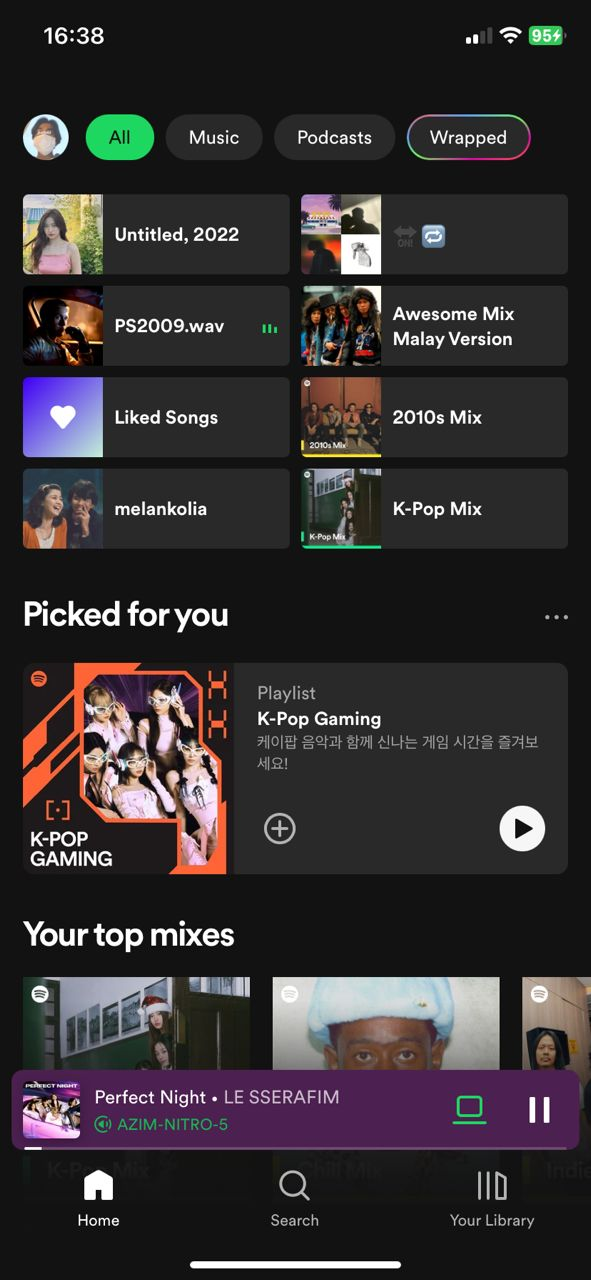
\includegraphics[width = \linewidth]{mainmatter/images/spotify1.jpg}
      \caption{Home Page}
      \label{fig:myfig17}
    \end{subfigure}%
    \hspace{1em}% Space between images A and B
    \begin{subfigure}{.3\linewidth}
      \centering
      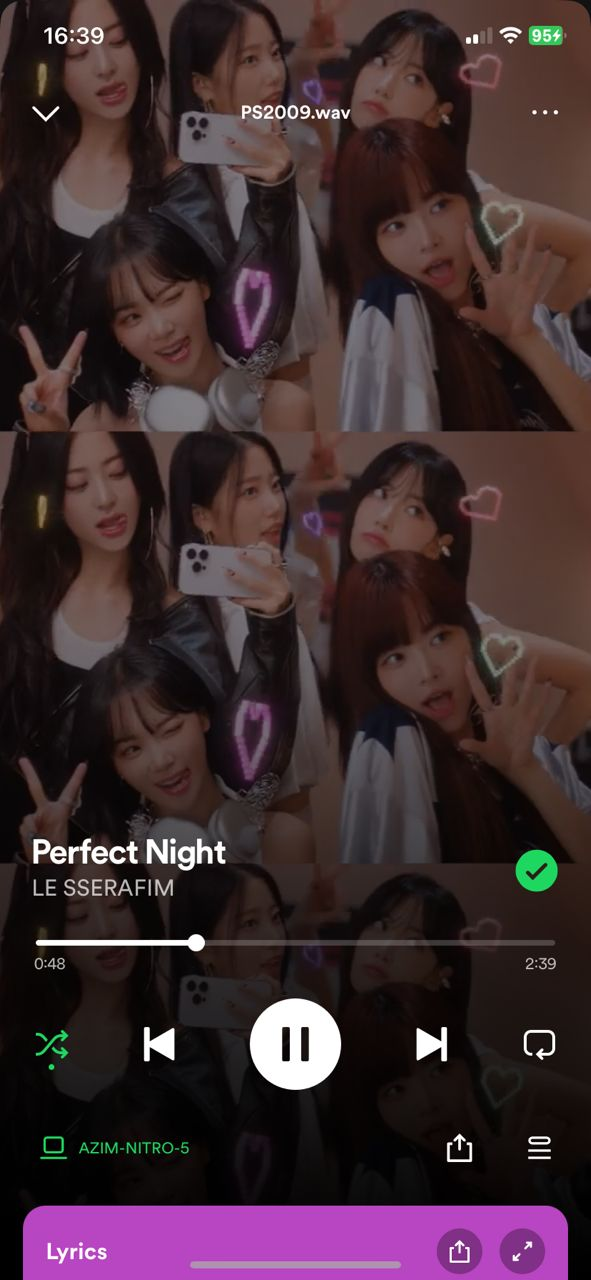
\includegraphics[width = \linewidth]{mainmatter/images/spotify2.jpg}
      \caption{Music Player}
      \label{fig:myfig18}
    \end{subfigure}%
    \hspace{1em}% Space between images B and C
    \begin{subfigure}{.3\linewidth}
      \centering
      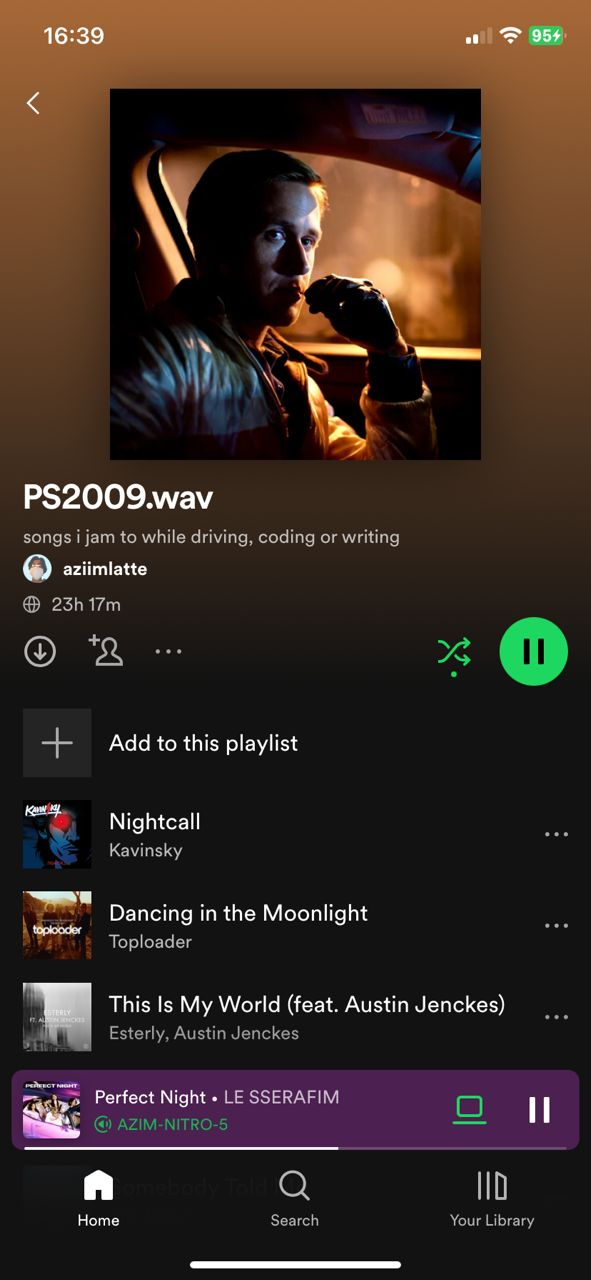
\includegraphics[width = \linewidth]{mainmatter/images/spotify3.jpg}
      \caption{Playlist Page}
      \label{fig:myfig19}
    \end{subfigure}
    \caption{Screenshots from Spotify Mobile Application}
    \caption*{\textit{Mobile Application Interface for Spotify [Spotify Technology S.A., 2024]}}
\end{figure}
Spotify is a famous music streaming platform that has transformed how individuals access and enjoy music on their mobile devices. The Spotify mobile app, accessible on Android and iOS platforms, provides an extensive collection of songs, albums, and playlists spanning diverse genres and artists. The application utilizes a freemium business model, offering users the choice to access a restricted version that includes intermittent adverts or upgrade to a premium membership for an uninterrupted experience without ads, along with supplementary functionalities like offline listening and higher audio quality. Spotify offers customers an intuitive and user-friendly interface that allows them to easily create and share playlists, explore new music based on personalized suggestions, and access a wide range of podcasts. \pagebreak
\begin{itemize}[\label{}]
    \item \textbf{Advantages} \\
    The mobile application of Spotify offers numerous benefits, making it a preferred option for music enthusiasts. The vast music collection offers millions of songs, catering to a wide range of musical preferences. The app utilizes personalized recommendation algorithms, such as Discover Weekly and Daily Mixes, to assist users in exploring new music that aligns with their listening tastes. The offline listening option is especially beneficial for customers who are frequently mobile since it enables them to download their preferred songs or playlists for playback without the need for an internet connection. Furthermore, Spotify's collaborative playlist function promotes social engagement by allowing friends to contribute to a shared playlist, thereby boosting the community experience of discovering music.
    \item \textbf{Limitations} \\
    Although widely used, the Spotify mobile application has limitations. An evident disadvantage for users who do not pay is the existence of advertisements, which might disrupt the pleasure of listening to music. Moreover, the availability of content on Spotify is subject to regional variations caused by licensing limitations, which restrict access to individual tracks or albums in some regions. Additionally, certain users have raised concerns regarding the remuneration system for artists on the platform, which relies on stream count and may potentially put smaller or independent bands at a disadvantage. Although the app provides an extensive music collection, many artists or albums may not be accessible due to licensing arrangements with record labels. Despite these limitations, Spotify maintains an outstanding position in the music streaming sector, consistently adapting to fulfill customer expectations.
\end{itemize}
\pagebreak

\subsection{Twitch}
\begin{figure} [h]
    \centering
    \begin{subfigure}{.3\linewidth}
      \centering
      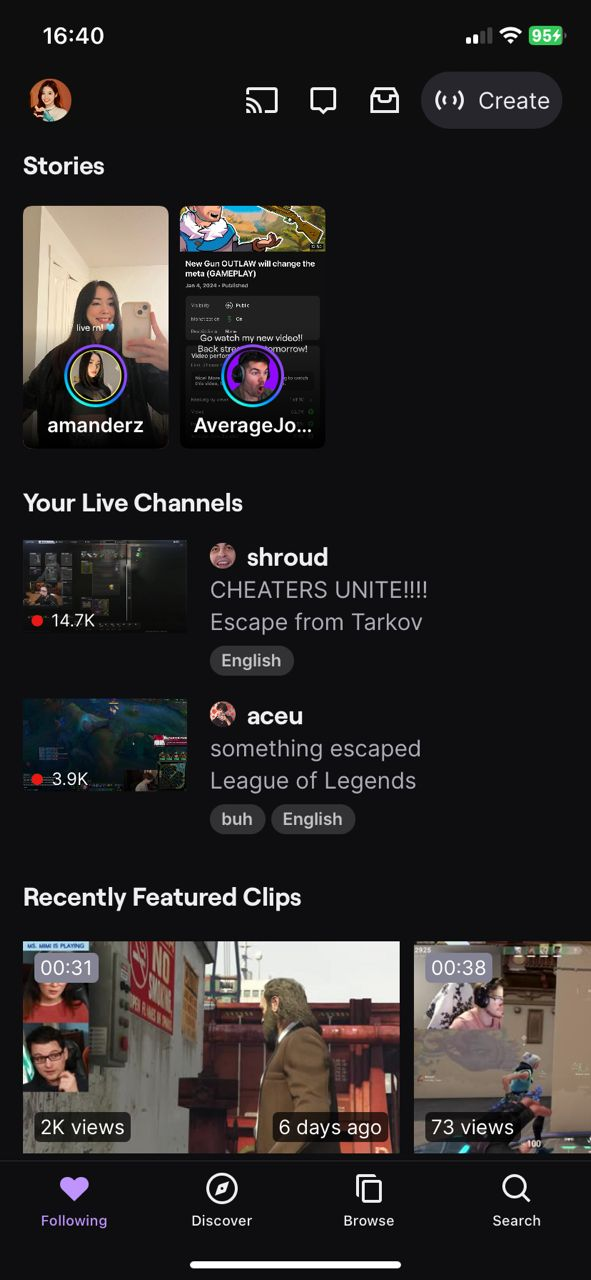
\includegraphics[width = \linewidth]{mainmatter/images/twitch1.jpg}
      \caption{Home Page}
      \label{fig:myfig20}
    \end{subfigure}%
    \hspace{1em}% Space between images A and B
    \begin{subfigure}{.3\linewidth}
      \centering
      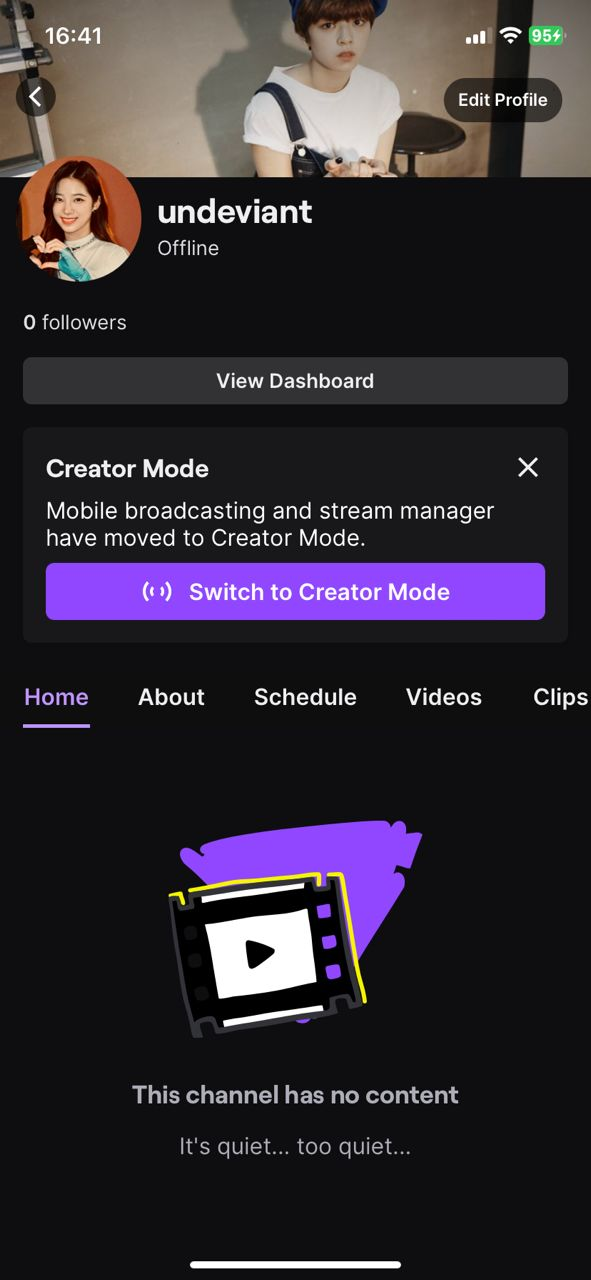
\includegraphics[width = \linewidth]{mainmatter/images/twitch2.jpg}
      \caption{User Profile}
      \label{fig:myfig21}
    \end{subfigure}%
    \hspace{1em}% Space between images B and C
    \begin{subfigure}{.3\linewidth}
      \centering
      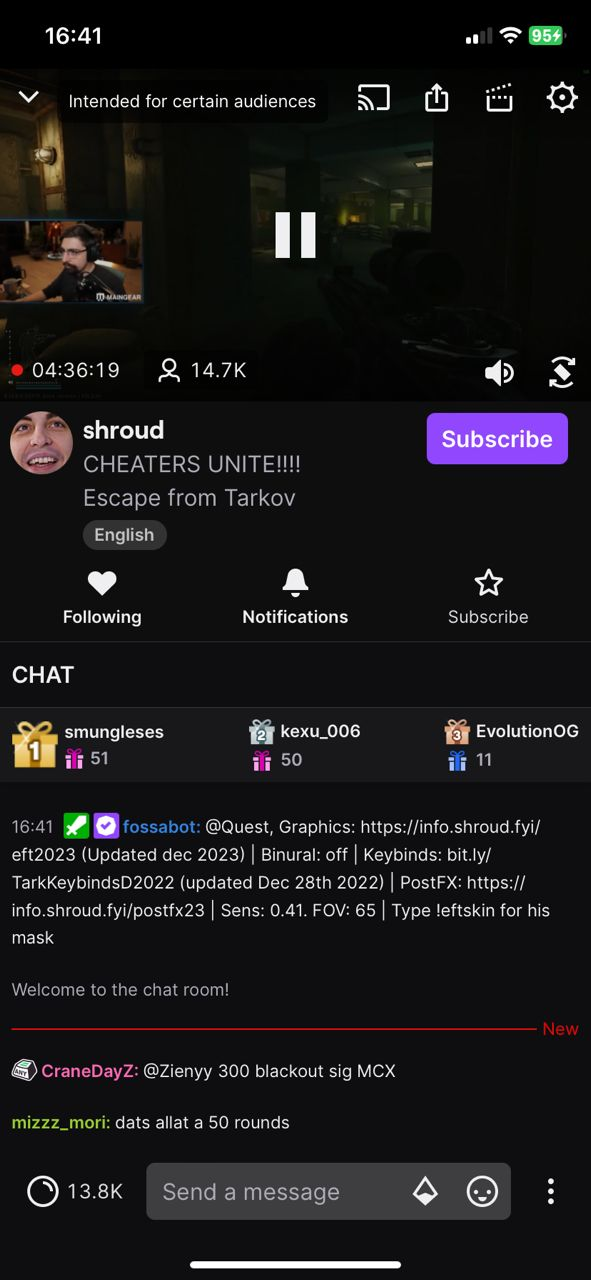
\includegraphics[width = \linewidth]{mainmatter/images/twitch3.jpg}
      \caption{Livestream Page}
      \label{fig:myfig22}
    \end{subfigure}
    \caption{Screenshots from Twitch Mobile Application}
    \caption*{\textit{Mobile Application Interface for Twitch [Amazon.com Inc., 2024]}}
\end{figure}
The Twitch mobile application, which is an essential component of the Twitch network, has experienced significant growth beyond its initial focus on gaming. Twitch, which was introduced in 2011, has expanded its scope beyond gaming and currently includes a diverse array of live streaming, such as music, talk shows, and creative content. The mobile application, accessible on both Android and iOS platforms, enables users to view real-time transmissions, interact with content creators through chat, and even initiate their live broadcasts directly from their mobile devices. During the COVID-19 epidemic, platforms such as Twitch played a vital role in facilitating connections among communities and providing assistance to video creators \parencite{leger21}. In addition to gaming, Twitch's mobile app functions as a flexible platform for content creators to live stream other forms of entertainment, such as music concerts, while also promoting a sense of community through instant interactions. \pagebreak
\begin{itemize}[\label{}]
    \item \textbf{Advantages} \\
    The mobile application offered by Twitch offers distinct benefits for content creators that aim to actively involve their viewers. The platform's unique monetization strategy, as highlighted by \textcite{leger21}, incorporates elements such as Bits, channel subscriptions, and donations, providing content creators with direct financial backing from their audience. This concept not only enables creators but also enables viewers to actively contribute to the long-term viability of their favorite channels. The mobile app's intuitive layout promotes effortless interaction, allowing users to effortlessly explore and endorse live streams. Additionally, interactive elements such as channel points and Bits enhance the entire viewer experience. The platform's advantages facilitate its role in revitalizing the music industry by establishing direct relationships between performers and their audiences.
    \item \textbf{Limitations} \\
    Although Twitch's mobile application provides an exciting platform for content makers, it does come with several difficulties. The platform encounters copyright-related challenges, as emphasized by \textcite{leger21}. Twitch, like other platforms, faces the continual challenge of effectively managing copyright concerns, particularly concerning music streaming. Another limitation is the necessity for a strong content control system to tackle improper or objectionable material. Furthermore, the mobile viewing experience may not offer the same level of engagement as larger displays, affecting the quality of interactions. Additionally, mobile viewers may encounter buffering or poor video quality in regions with weak signals, which might be a hindrance. Regardless of these challenges, Twitch continues to be a crucial platform, demonstrating the capacity for community-based models in the entertainment sector throughout extraordinary times.
\end{itemize}
\pagebreak

\subsection{Bandcamp}
\begin{figure} [h]
    \centering
    \begin{subfigure}{.3\linewidth}
      \centering
      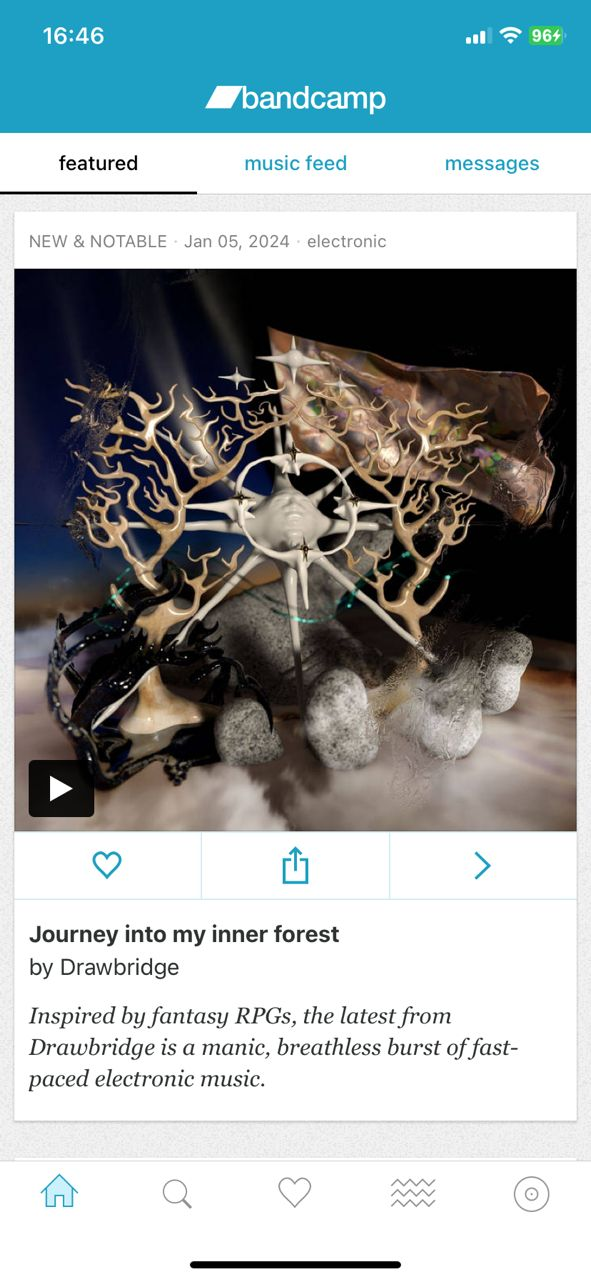
\includegraphics[width = \linewidth]{mainmatter/images/bandcamp1.jpg}
      \caption{Home Page}
      \label{fig:myfig23}
    \end{subfigure}%
    \hspace{1em}% Space between images A and B
    \begin{subfigure}{.3\linewidth}
      \centering
      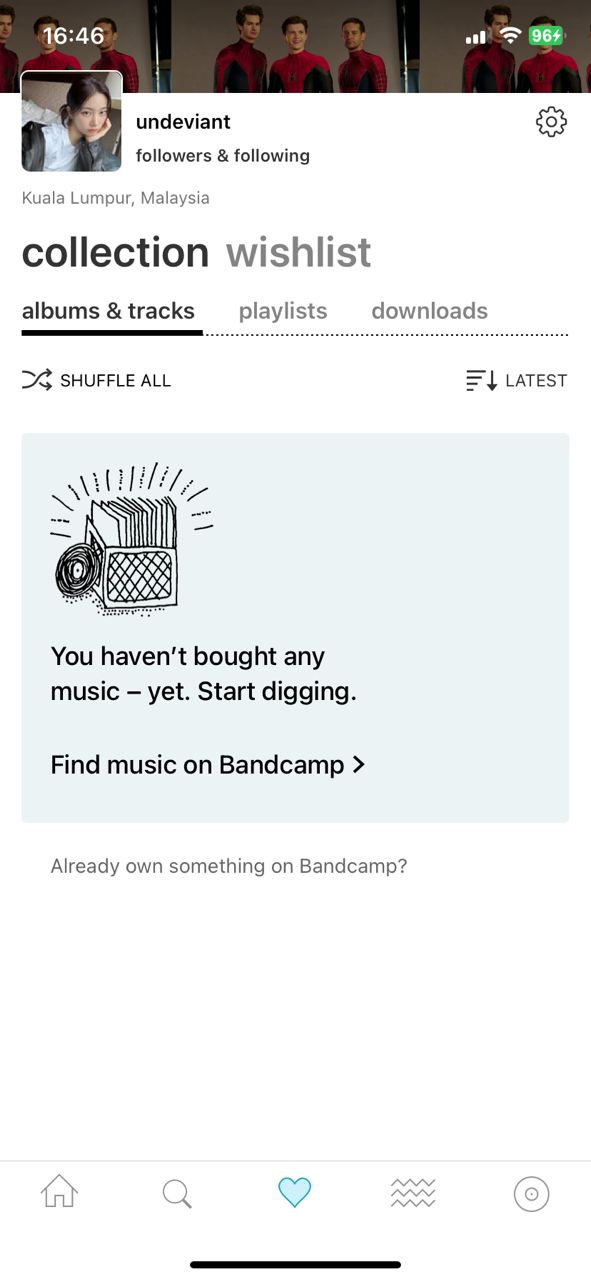
\includegraphics[width = \linewidth]{mainmatter/images/bandcamp2.jpg}
      \caption{User Profile}
      \label{fig:myfig24}
    \end{subfigure}%
    \hspace{1em}% Space between images B and C
    \begin{subfigure}{.3\linewidth}
      \centering
      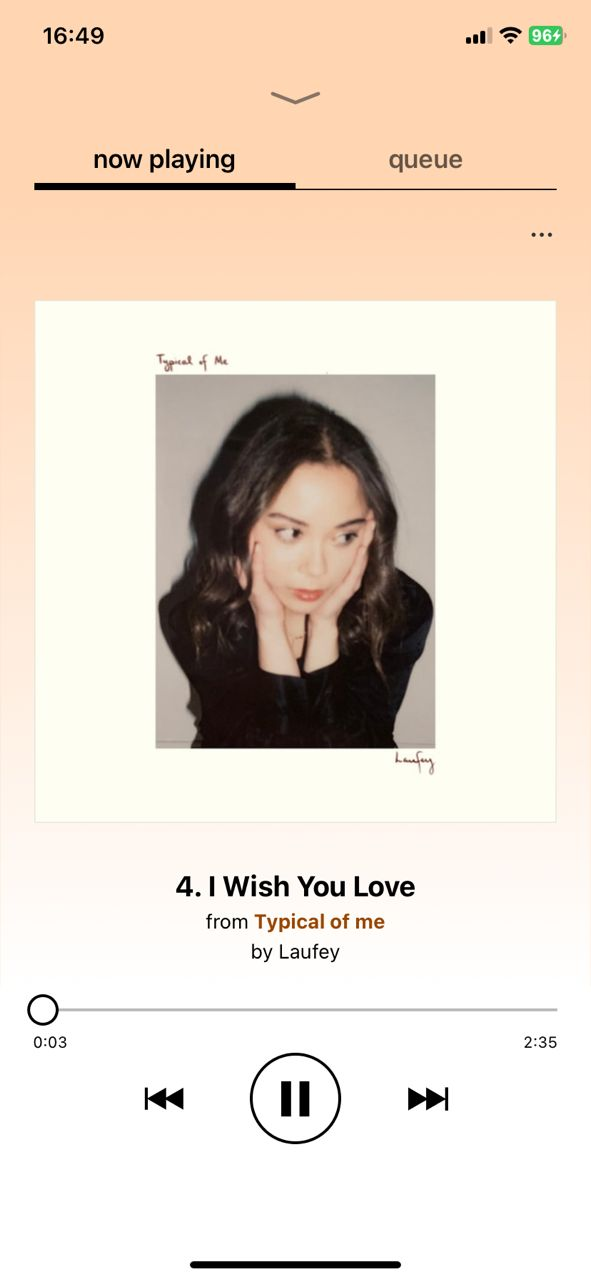
\includegraphics[width = \linewidth]{mainmatter/images/bandcamp3.jpg}
      \caption{Music Player}
      \label{fig:myfig25}
    \end{subfigure}
    \caption{Screenshots from Bandcamp Mobile Application}
    \caption*{\textit{Mobile Application Interface for Bandcamp [Songtradr, 2024]}}
\end{figure}
The Bandcamp mobile application, which was introduced in 2008, serves as a music platform that enables independent artists and labels to establish direct connections with their audience. It serves as a crucial platform in the music industry, following a community-driven approach examined by \textcite{leger21} among the difficulties posed by the COVID-19 epidemic. Bandcamp stands out for its focus on empowering independent musicians by enabling them to directly sell their albums and goods, rather than depending entirely on money from streaming. The platform's mobile application, accessible on Android and iOS, offers musicians a platform to organize their work, establish pricing, and directly engage with their fan base. This strategy enables artists to give priority to record and merchandise sales, which is a crucial factor in revitalizing the music industry by promoting community involvement \parencite{leger21}. \pagebreak
\begin{itemize}[\label{}]
    \item \textbf{Advantages} \\
    The mobile application of Bandcamp provides distinct benefits that align with the community-oriented framework proposed by \textcite{leger21}. The platform's emphasis on record and product sales enables artists to gain more control over their revenue streams and forge a more intimate bond with their audience. Users of the platform not only operate as consumers, but also are passionate supporters, as Bandcamp empowers them to make payments exceeding the predetermined price for songs, directly support their preferred artists, and take part in events such as Bandcamp Fridays. The mobile application acts as a direct channel for this interaction, offering users a customized and artist-focused encounter, strengthening the feeling of connection between musicians and their supporters.
    \item \textbf{Limitations} \\
    The Bandcamp mobile application exhibits limitations that mirror the difficulties encountered by platforms emphasized by \textcite{leger21}, despite having significant qualities. The platform's dependence on album sales could provide difficulty in terms of being easily found, as Bandcamp may not provide the same algorithm-based suggestions as popular streaming services. The app's UI, albeit functional, may lack the refinement and extensive features found in larger platforms. In addition, the direct-to-fan technique employed by Bandcamp may restrict access to specific mainstream or major-label content, so impacting users who desire a broader range of music options. However, the platform's dedication to creating a direct and supportive connection between artists and their fan base overcomes these limitations.
\end{itemize}
\pagebreak

\subsection{SoundCloud}
\begin{figure} [h]
    \centering
    \begin{subfigure}{.3\linewidth}
      \centering
      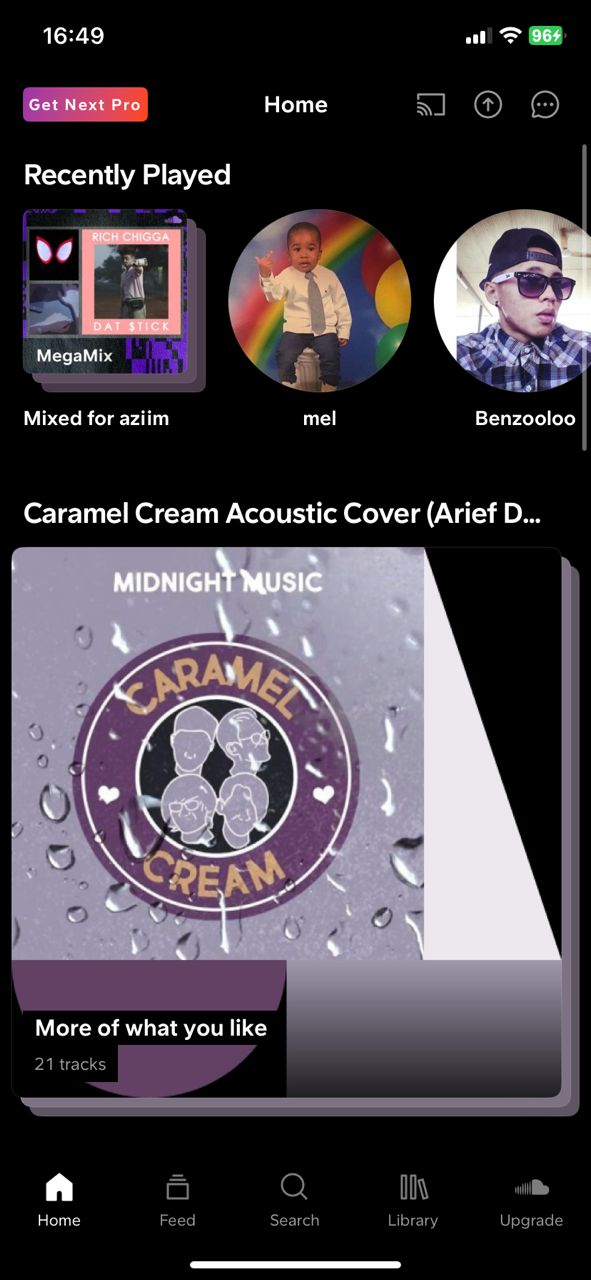
\includegraphics[width = \linewidth]{mainmatter/images/soundcloud1.jpg}
      \caption{Home Page}
      \label{fig:myfig26}
    \end{subfigure}%
    \hspace{1em}% Space between images A and B
    \begin{subfigure}{.3\linewidth}
      \centering
      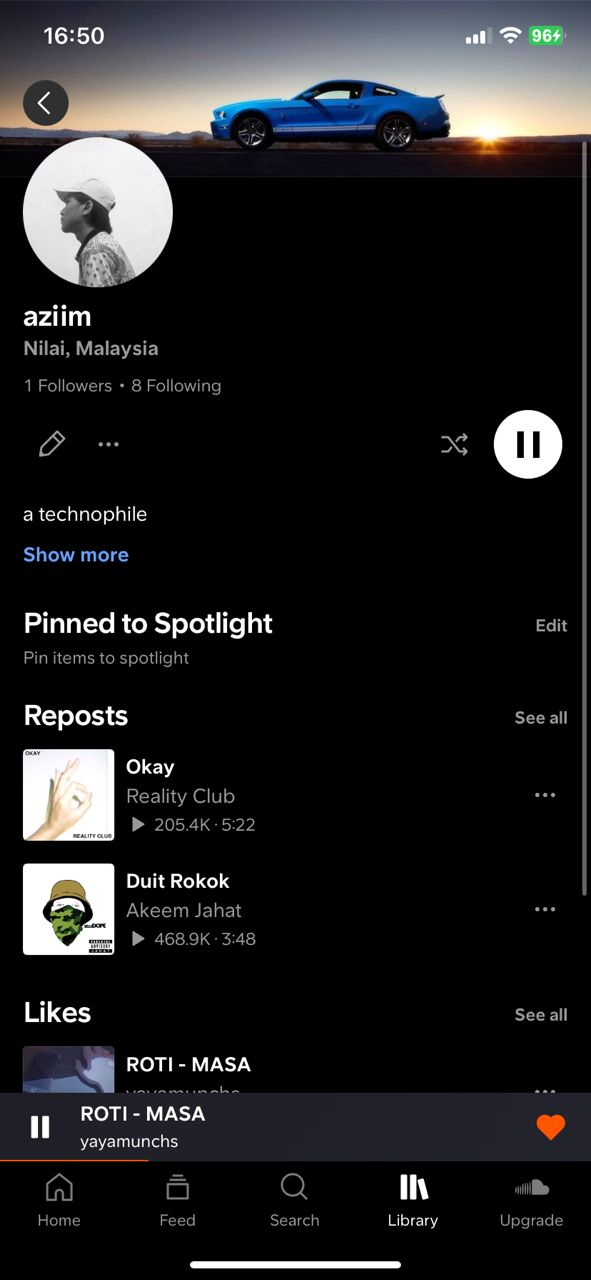
\includegraphics[width = \linewidth]{mainmatter/images/soundcloud2.jpg}
      \caption{User Profile}
      \label{fig:myfig27}
    \end{subfigure}%
    \hspace{1em}% Space between images B and C
    \begin{subfigure}{.3\linewidth}
      \centering
      
\includegraphics[width = \linewidth]{mainmatter/images/soundcloud3.jpg}
      \caption{Music Player}
      \label{fig:myfig28}
    \end{subfigure}
    \caption{Screenshots from SoundCloud Mobile Application}
    \caption*{\textit{Mobile Application Interface for SoundCloud [SoundCloud, 2024]}}
\end{figure}
SoundCloud is a unique and extensively utilized mobile application that specifically emphasizes music material created by users. Introduced in 2007, the website enables musicians, producers, and fans to publish, distribute, and explore a wide array of audio content, encompassing music tracks, podcasts, and sound snippets. The SoundCloud mobile app, accessible on Android and iOS devices, offers users an extensive and diverse collection of music that encompasses a wide range of genres and styles. The platform's interface is specifically built to facilitate effortless navigation and exploration. As a result, it has become a popular choice for up-and-coming musicians who are hoping to gain attention, as well as for listeners who are interested in discovering new and often unconventional music. \pagebreak
\begin{itemize}[\label{}]
    \item \textbf{Advantages} \\
    SoundCloud has numerous benefits, which contribute to its popularity among music enthusiasts. The online platform functions as an entry point for up-and-coming and independent artists, enabling them to showcase their artistic works to a worldwide audience. The application's social functionalities, such as the ability to leave comments and express approval through likes on music recordings, enable direct engagement between artists and fans, establishing a sense of communal connection. SoundCloud's recommendation algorithms promote the exploration of new music that is customized to users' preferences. Additionally, the platform's open and democratic environment fosters inclusiveness for creators of all skill levels. Furthermore, the app's free version offers an extensive amount of material without necessitating a subscription, rendering it accessible to a wide range of users.
    \item \textbf{Limitations} \\
    Although SoundCloud offers notable benefits it also encounters particular limitations. An issue arises from the disparity in audio quality among songs because the content is created by users and may differ in terms of production standards. The platform's complimentary edition is financed by adverts, and certain users may perceive the frequency of commercials as disruptive to their listening experience. Another constraint is the possibility of copyright infringement problems, as the unrestricted nature of the platform may result in the dissemination of unauthorized content. In addition, the extensive collection of music on SoundCloud can occasionally provide a challenge for users to find top-notch content amidst a large number of uploads. Furthermore, the lack of a complete catalog of popular music from major record labels may be a disadvantage for individuals looking for more mainstream songs. Notwithstanding these constraints, SoundCloud continues to be a prominent contender in the realm of online music streaming, especially for individuals who prioritize variety and active participation in their music exploration.
\end{itemize}
\pagebreak

\subsection{IMDb}
\begin{figure} [h]
    \centering
    \begin{subfigure}{.3\linewidth}
      \centering
      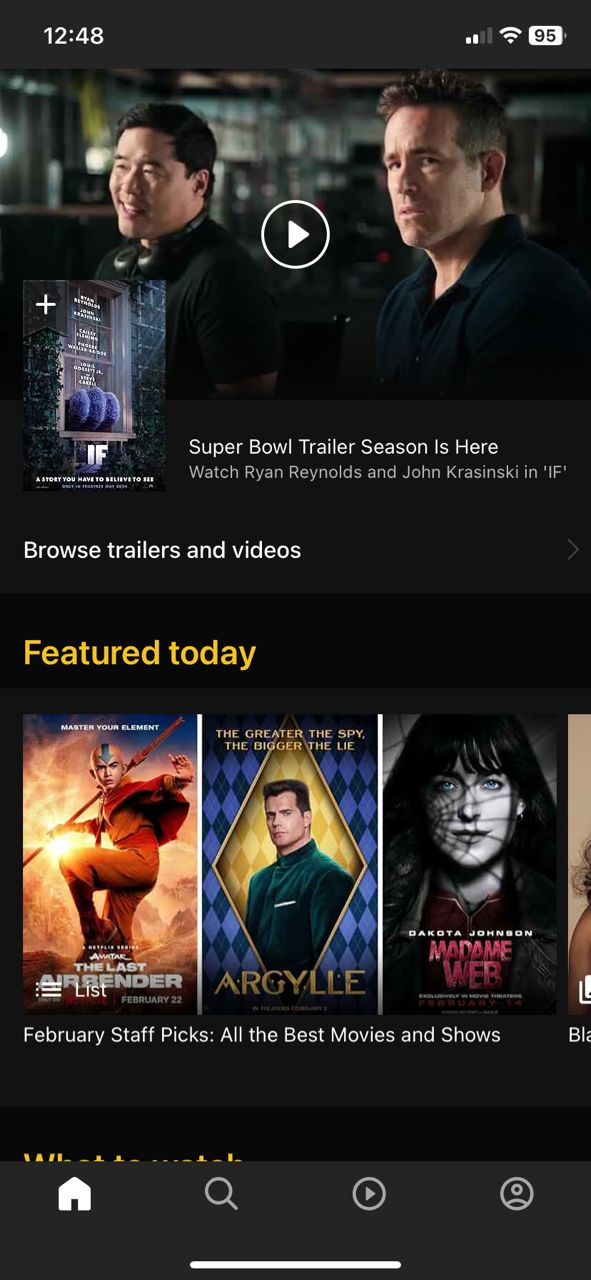
\includegraphics[width = \linewidth]{mainmatter/images/imdb1.jpg}
      \caption{Home Page}
      \label{fig:myfig29}
    \end{subfigure}%
    \hspace{1em}% Space between images A and B
    \begin{subfigure}{.3\linewidth}
      \centering
      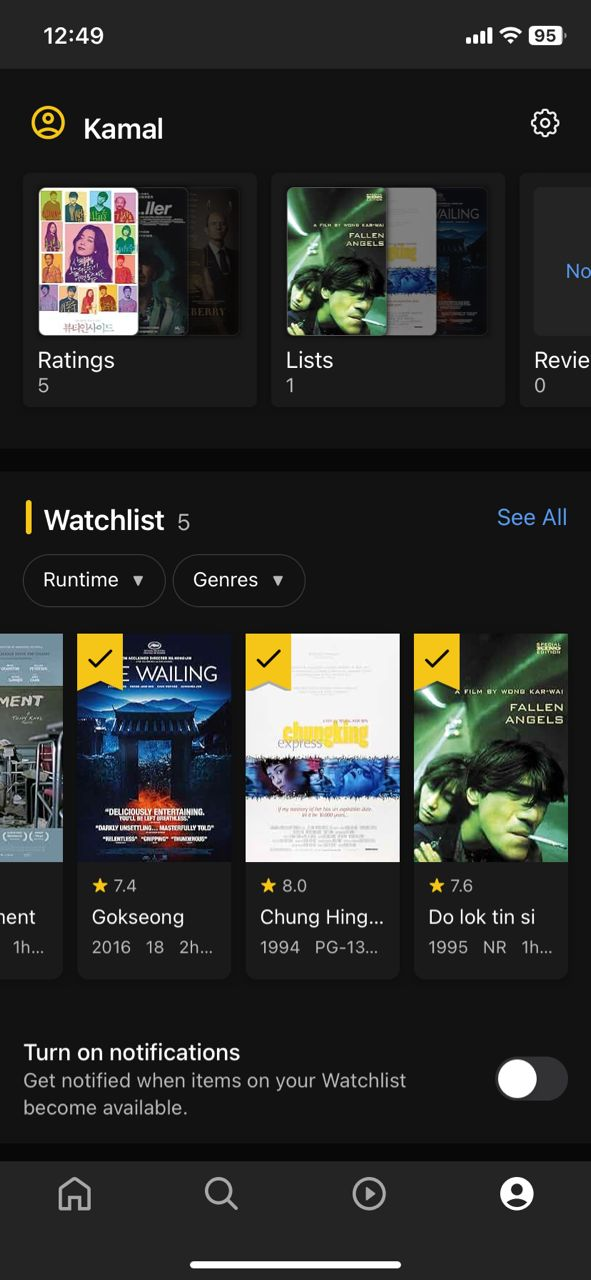
\includegraphics[width = \linewidth]{mainmatter/images/imdb2.jpg}
      \caption{User Profile}
      \label{fig:myfig30}
    \end{subfigure}%
    \hspace{1em}% Space between images B and C
    \begin{subfigure}{.3\linewidth}
      \centering
      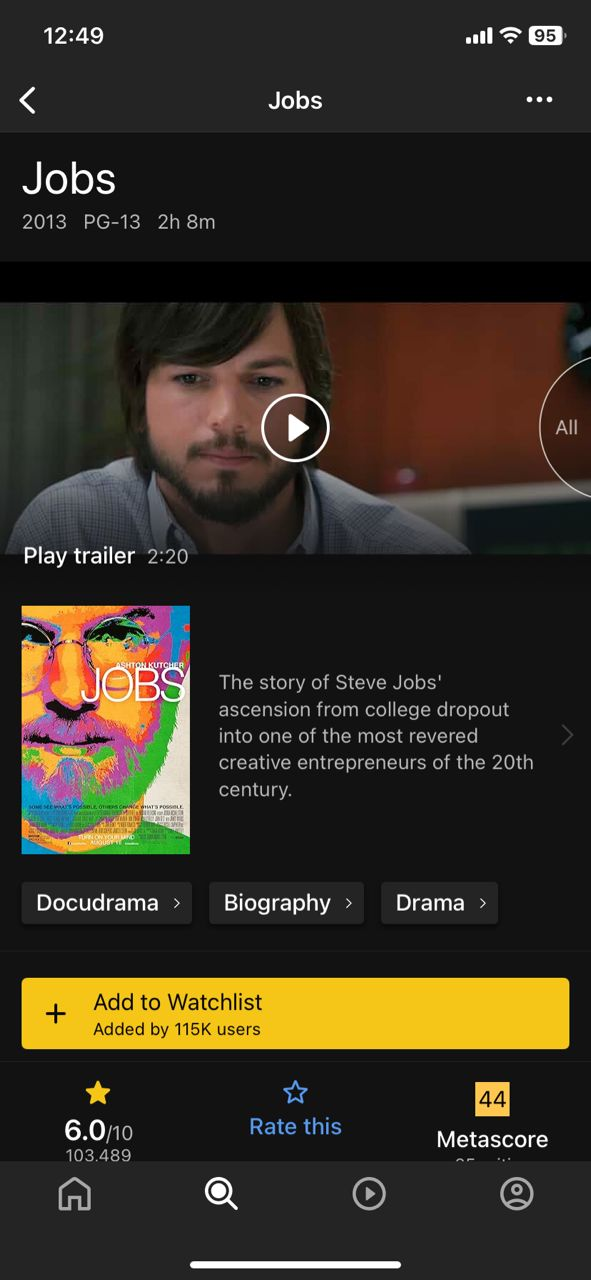
\includegraphics[width = \linewidth]{mainmatter/images/imdb3.jpg}
      \caption{Film Page}
      \label{fig:myfig31}
    \end{subfigure}
    \caption{Screenshots from IMDb Mobile Application}
    \caption*{\textit{Mobile Application Interface for IMDb [Amazon.com Inc., 2024]}}
\end{figure}
The IMDb mobile application is a comprehensive and user-friendly platform designed for movie fans and TV series enthusiasts. The platform provides a wide library of data regarding films, TV series, actors, and production staff, allowing users easy access to comprehensive information about their preferred entertainment content. Users can navigate through comprehensive catalogs of films and television shows, see previews, explore critics, and uncover the most recent updates in the entertainment sector. Moreover, the application offers personalized functionalities such as the ability to rate and review films, create watchlists, and receive recommendations tailored to user interests. This makes it a valuable companion for individuals who are enthusiastic about the worlds of cinema and television. \pagebreak
\begin{itemize}[\label{}]
    \item \textbf{Advantages} \\
    The IMDb mobile application provides a wide range of benefits to its users. Firstly, it offers instant access to a vast constantly updated library of films, television programs, and details about celebrities, rendering it a crucial resource for fans of entertainment. Users may efficiently access information, evaluations, and rankings for films and TV shows, facilitating well-informed choices when selecting what to watch. The app's customized functionalities, such as watchlists and personalized suggestions, enhance the user experience by enabling the discovery of material that is similar to their tastes. Moreover, IMDb's incorporation with streaming sites enables users to conveniently locate the platforms on which they may watch their preferred episodes and films, thus simplifying their entertainment options. Overall, the IMDb mobile app is a useful and essential tool for both film enthusiasts and television lovers.
    \item \textbf{Limitations} \\
    A disadvantage of the IMDb mobile application is the inclusion of advertisements and promotional material, which can occasionally interrupt the user's experience and provide distractions while searching for information or reading reviews. In addition, the application might require a reliable internet connection to access its functionalities and database, which can be troublesome for users residing in regions with restricted connectivity. In addition, IMDb offers a vast amount of information, but it depends on user-generated content for ratings and reviews, which may sometimes be subjective or unreliable. Finally, certain users can see the interface as crowded or overwhelming because of the substantial quantity of data displayed, thus leading to less natural navigation for beginners to the site.
\end{itemize}
\pagebreak

\subsection{Summary of Comparison between Existing Mobile Applications}
\begin{longtable}{|p{2.2cm}|p{1.8cm}|p{1.5cm}|p{1.5cm}|p{1.8cm}|p{1.8cm}|p{1.5cm}|}
\caption{Comparison between Existing Mobile Applications} 
\label{tab:alongtable} \\

\hline
\textbf{Existing Apps} & \multicolumn{1}{c|}{\textit{Letterboxd}} & \multicolumn{1}{c|}{\textit{Spotify}} & \multicolumn{1}{c|}{\textit{Twitch}} & \multicolumn{1}{c|}{\textit{Bandcamp}} & \multicolumn{1}{c|}{\textit{SoundCloud}} & \multicolumn{1}{c|}{\textit{IMDb}}\\
\hline 
\endfirsthead

% Table data
\textbf{Platform} & iOS \& Android & iOS \& Android & iOS \& Android & iOS \& Android & iOS \& Android & iOS \& Android \\ \hline
\textbf{Language} & English & English & English & English & English & English \\ \hline
\multicolumn{6}{|l|}{\textbf{Features}} \\ \hline
\textbf{User Verification} & \multicolumn{1}{c|}{\checkmark} & \multicolumn{1}{c|}{\checkmark} & \multicolumn{1}{c|}{\checkmark} & \multicolumn{1}{c|}{\checkmark} & \multicolumn{1}{c|}{\checkmark} & \multicolumn{1}{c|}{\checkmark} \\ \hline
\textbf{User Profile} & \multicolumn{1}{c|}{\checkmark} & \multicolumn{1}{c|}{\checkmark} & \multicolumn{1}{c|}{\checkmark} & \multicolumn{1}{c|}{\checkmark} & \multicolumn{1}{c|}{\checkmark} & \multicolumn{1}{c|}{\checkmark} \\ \hline
\textbf{Content Snippet Sharing} & & \multicolumn{1}{c|}{\checkmark} & & & \multicolumn{1}{c|}{\checkmark} & \\ \hline
\textbf{Favourite or Bookmark} & \multicolumn{1}{c|}{\checkmark} & \multicolumn{1}{c|}{\checkmark} & \multicolumn{1}{c|}{\checkmark} & \multicolumn{1}{c|}{\checkmark} & \multicolumn{1}{c|}{\checkmark} & \multicolumn{1}{c|}{\checkmark} \\ \hline
\textbf{Ratings or Review} & \multicolumn{1}{c|}{\checkmark} & & & & & \multicolumn{1}{c|}{\checkmark} \\ \hline
\textbf{Social Media Integration} & \multicolumn{1}{c|}{\checkmark} & \multicolumn{1}{c|}{\checkmark} & \multicolumn{1}{c|}{\checkmark} & & \multicolumn{1}{c|}{\checkmark} & \\ \hline
\textbf{Premium Plans} & \multicolumn{1}{c|}{\checkmark} & \multicolumn{1}{c|}{\checkmark} & \multicolumn{1}{c|}{\checkmark} & \multicolumn{1}{c|}{\checkmark} & \multicolumn{1}{c|}{\checkmark} & \multicolumn{1}{c|}{\checkmark} \\ \hline
\end{longtable}

When comparing Letterboxd, Spotify, Twitch, Bandcamp, and SoundCloud across multiple aspects, it becomes apparent that each site caters to distinct types of content and user engagements. All five services offer specialized applications for both iOS and Android, ensuring comprehensive accessibility across platforms. The language support is uniformly provided in English, ensuring constant user engagement and comprehension of the information. \pagebreak

These platforms include standardized authentication elements that necessitate users to create accounts to have personalized experiences. User profiles are a prevalent characteristic that enables individuals to showcase their preferences and engagement within the community. Content snippet sharing is widespread on platforms like Spotify and SoundCloud, allowing users to easily share their favorite snippets from media with others. Although many platforms provide a favorite or bookmark function for users to organize their selected material, the details may differ. Letterboxd specializes in films, Spotify specializes in music, Twitch specializes in live broadcasts, Bandcamp specializes in music and merchandise, and SoundCloud specializes in user-generated audio material. \\

On Letterboxd, ratings and reviews play a crucial role in evaluating films, offering a significant means of receiving feedback. The integration of social media is highly effective on various platforms, except Bandcamp, enabling users to effortlessly send their activity on other platforms. Subscription models vary depending on the type of content. Spotify, Twitch, and SoundCloud provide premium memberships that eliminate ads and offer extra functionality. On the other hand, Letterboxd and Bandcamp operate on a freemium model, where users have the option to subscribe for improved services or to support the site. These platforms essentially demonstrate the variety in how material is consumed, how users interact, and the different ways businesses operate in the fields of films, music, and live streaming.